% Template for ICIP-2015 paper; to be used with:
%          spconf.sty  - ICASSP/ICIP LaTeX style file, and
%          IEEEbib.bst - IEEE bibliography style file.
% --------------------------------------------------------------------------
\documentclass{article}
\usepackage{spconf,amsmath,graphicx}
\usepackage{tikz}
\usetikzlibrary{shapes.geometric, arrows}
% Example definitions.
% --------------------
\def\x{{\mathbf x}}
\def\L{{\cal L}}

% Title.
% ------
\title{V151231: NEAR EARTH BODY DETECTION and linking}
%
% Single address.
% ---------------
\name{ us the authors us the authors us the authors 
\thanks{This work is supported by NASA Grant XYZ.}}
\address{The Johns Hopkins University  \\ $^{1}$Dept. of Computer Science, $^{2}$Dept. of Applied Mathematics and Statistics, $^{3}$Applied Physics Laboratory}
%
% For example:
% ------------
%\address{School\\
%	Department\\
%	Address}
%
% Two addresses (uncomment and modify for two-address case).
% ----------------------------------------------------------
%\twoauthors
%  {A. Author-one, B. Author-two\sthanks{Thanks to XYZ agency for funding.}}
%	{School A-B\\
%	Department A-B\\
%	Address A-B}
%  {C. Author-three, D. Author-four\sthanks{The fourth author performed the work
%	while at ...}}
%	{School C-D\\
%	Department C-D\\
%	Address C-D}
%
\begin{document}
%\ninept
%
\maketitle
%
\begin{abstract}
While most asteroid population discovery to-date has been accomplished  by earth-based telescopes, it is speculated that most of the smaller Near Earth Objects (NEOs), up to 140 meters in diameter, whose impact can create substantial city-size damage, have not yet been discovered.  Further, there are asteroids that cannot be detected with an earth-based telescope given their size or the location of the Sun.  Our objective is therefore to develop an efficient asteroid detection and identification algorithm that can be hosted on-board a spacecraft.  By having on-board algorithms, the system would also minimize the need to downlink entire images taken by a space-based telescope. We describe one such image processing pipeline we have developed for asteroid detection and also characterize its performance.
 
\end{abstract}
%
\begin{keywords}
Asteroids detection, identification. 
\end{keywords}
%
\section{Introduction}
\label{sec:intro}

NASA has a congressional mandate to discover all Near-Earth Objects (NEOs) at least 1 kilometer in diameter.  Fortunately, 95\% of the NEOs larger than 1 km that have been discovered are likely not to impact Earth.  
Near-Earth Object search programs~\cite{stokes2002near} are currently almost exclusively accomplished by earth-based telescopes such as MIT's LINEAR \cite{evans2003detection}  project, the NEAT~\cite{neat2014} program, the Catalina Sky Survey, or  Pan-STARRS~\cite{denneau2013pan}.  (An exception is JPL's spacecraft-based WISE telescope brought out of hibernation to characterize NEOs in the 3.4 and 4.6 micron infrared bands~\cite{wise2014}). 

It is notable however that the NEO that has impacted Chelyabinsk, Russia on 15 February 2013 was only about 17 meters in size.  The impact of a 50 meter asteroid that caused the Tunguska Event of 1908 could have destroyed an entire city or metropolitan area. It is estimated that only a relatively small fraction of those so called ``city-killing'' asteroids, particularly objects less than 140 meters in diameter, have been discovered to date. Because of their size, atmospheric effects and the location of the sun, some of these NEOs cannot easily be detected with an earth-based telescope.  

Our focus here is therefore on developing an algorithm that can be hosted on-board a spacecraft.  Understanding that there are processing and resources (memory) constraints on-board, our algorithm design needs to not only meet the performance objectives of detecting and identifying asteroids using a space-based telescope, but it also needs to have a small footprint to be implementable with the limited on-board resources.  This paper describes an agile algorithm candidate that is being investigated as well as our use of representative space-based imagery for testing it.

There is prior image analysis work for asteroid detection for ground-based image observations. In~\cite{denneau2013pan}, a reference processing system for detection and identification of asteroid is reported, named the Pan-STARRS Moving Object Processing System (MOPS). This pipeline aims at identifying moving objects in our solar system and linking those detections within and between night observations. It attributes those detections to known objects, calculates initial and differentially corrected orbits for linked detections, recovering detections when they exist, and orbit identification. Most proposed pipelines for earth based detection include a step to combine together images to create a high S/N static-sky image that is subtracted from the current master image to obtain a difference image containing only transient sources. Examples include \cite{shao2014finding}, where a shift-and-add technique is used to improve  signal to noise ratio and then synthetically creating long exposure images to facilitate the detection of trajectories. A related shift-and-add method using a median  image rather than an average image is reported in~\cite{yanagisawa2005automatic}. A match filter is used for asteroid detection and matching in \cite{gural2005matched}. In \cite{kubica2005variable,kubica2005multiple,kubica2007efficient}, tree based searches (including KD-trees) are used for efficient linking of successive asteroids detections and finding sets of observation points that can be fitted with an inherent motion model, through an exhaustive search for all possible linkages that satisfy the expected model constraints.
	
In Section~\ref{sec:approach} we describe an agile pipeline that can be deployed on an on board system. This approach is both small-footprinted and efficient, and uses Principal Component Analysis rather than tree-based searches to aggregate object detections into trajectories. Since on-board surveys are not available we describe in Section~\ref{sec:experiments} how we validate and test our method using simulated images as well as earth based and space-based image datasets that contain associated ground truth.

\section{Approach}
\label{sec:approach}

We describe the main components of our image processing pipeline (shown also in the flow chart in figure \ref{IPP}) addressing detection and linking of asteroids seen in images acquired from space-based platforms.  At a high level, the pipeline is summarized as follows: as input to the pipeline is a sequence of time-lapse images. Pre-processing and image registration are used to bring the images into alignment with a common image of reference.  Detection of bright bodies is done via thresholding, followed by logical differencing between each image and a reference image containing objects that are common to all registered images in the sequence of images.  After differencing, which allows us to detect moving objects, we use an additional step to filter detections based on size and shape considerations (using tools such as connected components and morphological filters).  A list of detection coordinates is then generated.  Candidate trajectories are then generated for these coordinates by checking rectilinearity (via Principal Component Analysis).  A last verification step further checks additional conditions such as the fact that candidate trajectories must be composed of temporally consecutive mover observations.  Each module that is detailed next. 

\tikzstyle{block} = [rectangle, minimum width=1.8cm, minimum height=1.5cm, text centered, text width=1.8cm, draw=black, fill=blue!15]
\tikzstyle{arrow} = [thick,->,>=stealth]
\begin{figure}[b]
\begin{tikzpicture}[node distance=2.25cm]
\node (proc) [block] {Image Pre-Processing};
\node (reg) [block, right of=proc] {Image Registration};
\node (diff) [block, right of=reg] {Logical Differencing};
%\node (det) [block, right of=diff, yshift=1.2cm] {Trajectory Detection};
\node (det) [block, right of=diff] {Trajectory Detection};
\draw [arrow] (proc) -- (reg);
\draw [arrow] (reg) -- (diff);
\draw [arrow] (diff) -- (det);
\end{tikzpicture}
\vspace{-0.7cm}
\caption{Image Processing Pipeline}
\label{IPP}
\end{figure}

{\bf Image Pre-Processing}
We standardize the input images by using a series of photometric and geometric transformations.  This includes employing techniques to reduce noise (e.g. median filter) and artifacts that are consequences of the intrinsic properties of the acquisition device.   This coordinate information can then be stored in the FITS (Flexible Image Transport System) image header for later use in the Trajectory Verification stage.

{\bf Image Registration}
Image registration refers to finding the transformation that would align multiple images of the same scene that are obtained at different times from slightly different viewpoints.  We aim to align each image in the sequence to a common reference image so that the stars in the background line up in all images.  In the case of a triplet of images, typically the second image is used as the reference image.  We estimate and then apply the necessary translation, rotation, scaling (similarity transformation) and/or skew (full affine transformation) to all images in the sequence such that image objects (stars) are mapped into the same pixels location and so that all transformed images have the same spatial resolution.  Image Registration using mutual information~\cite{viola1997alignment} and cross-correlation as similarity measures are used. 

{\bf Image Logical Differencing}
A global thresholding is applied to the registered image for detecting asteroids and suppressing background noise.  As asteroids are typically very faint compared to the surrounding stars, the selection of the detection threshold impacts false alarm rate.  Thresholding yields binary detection images.  The set of all binary images is then used to generate an intersection image that contains objects that occur in all images in the sequence.  This is followed by logical differencing whereby we produce a set of difference images by intersecting the corresponding binary image with the negative of the common intersection image.  This operation provides a list of candidate detections for each image in the sequence.  While the logical differencing results in good detections, additional artifacts such as crater-like formations are seen as a result of some of the celestial bodies being over-exposed.  To mitigate this artifact, we subsequently perform filtering out of hollow objects as well as filtering based on object size.

{\bf Trajectory Detection}
The list of centroids of moving objects obtained from image differencing defines a set of candidate rectilinear trajectories.  The goal is to find a subset of centroids that fit a linear model. Even though the model is simple, the set of filtered centroids potentially has a high number of noisy points (falsely detected movers), and the cardinality of the set of all candidate trajectories increases exponentially with the number of detections, thus requiring subsequent pruning of this set.  We search through all possible trajectories via Principal Component Analysis (PCA) and compute the ratio of eigenvalues, $\lambda_{1}/(\lambda_{1}+ \lambda_{2})$ in order to develop a line confidence score for each candidate trajectory, and choose candidate lines for which this ratio exceeds a threshold. Using the candidate trajectories thus found, we then enforce temporal order of detection by using the sign of the projection on the principal eigenvector.  As the final step, we further eliminate false positives by ensuring that the distance between projections is proportional to the time interval between images.  

{\bf Trajectory Detection(PCA+Tree) - Phil: I added this so that we can talk about this tomorrow. This needs more work.}
The list of centroids of moving objects obtained from image differencing defines a set of candidate rectilinear trajectories.  The goal is to find a subset of centroids that fit a linear model. Even though the model is simple, the set of filtered centroids potentially has a high number of noisy points (falsely detected movers), and the cardinality of the set of all candidate trajectories increases exponentially with the number of detections, thus requiring subsequent pruning of this set. We use a combination of Principal Component Analysis (PCA) and 2d-trees in order to find the trajectories efficiently. Unlike MOPS and CSS(TODO: Add Catalina reference, find the name of their pipeline), we do not set an upper limit on the velocity of the asteroid, and hence do not miss potential fast moving targets. Given a sequence of images, we form all the possible trajectories connecting the detections in the first and last frames. There are $O(n^2)$ trajectories, where $n$ is the number of detections per images. We then find the point of intersection of each of these trajectories with the frames in the middle. We construct a 2 dimensional tree for all the frames in the middle, and perform a range search on the tree to give us the detections that lie within a small radius of the point of intersection. This query can be done on $O(log(n))$ time on average. Once we find a collection of such points that potentially form a linear trajectory, we perform PCA and compute the ratio of eigenvalues, $\lambda_{1}/(\lambda_{1}+ \lambda_{2})$ in order to develop a line confidence score for each candidate trajectory, and choose lines for which this ratio exceeds a threshold. Using the candidate trajectories thus found, we then enforce temporal order of detection by using the sign of the projection on the principal eigenvector.  As the final step, we further eliminate false positives by ensuring that the distance between projections is proportional to the time interval between images. Compared to a brute force line search($O(n^k)$, where $k$ is the number of images in the sequence) our algorithm takes $O(n^2log(n))$ time. (TODO: Verify this.)

% !TEX root = main.tex
\section{Experiments}
%\section{Experiments}
%\label{sec:experiments}
%
%\subsection{Simulated Imagery}
%\label{ssec:simulated}
%
%\subsection{Real Imagery}
%\label{ssec:real}
%
%\subsubsection{NEAT}
%\subsubsection{CATALINA}
%
%
%\subsection{performance characterization}

\label{sec:experiments}

We detail the experiments performed using a range of simulated space-based imagery generated using the JHU/APL developed {\em Renderer and Camera Emulator} (RCE) as well as real imagery from the NEAT dataset.  

%We  detail experiments using a JHU/APL developed Renderer and Camera Emulator (RCE) to simulate a range of imagery and real imagery from the NEAT dataset.  

%
\begin{figure}[t]
\vspace{-0.3cm}
\begin{center}$
\begin{array}{@{\hspace{0.2em}}c@{\hspace{0.2em}}c@{\hspace{0.2em}}}
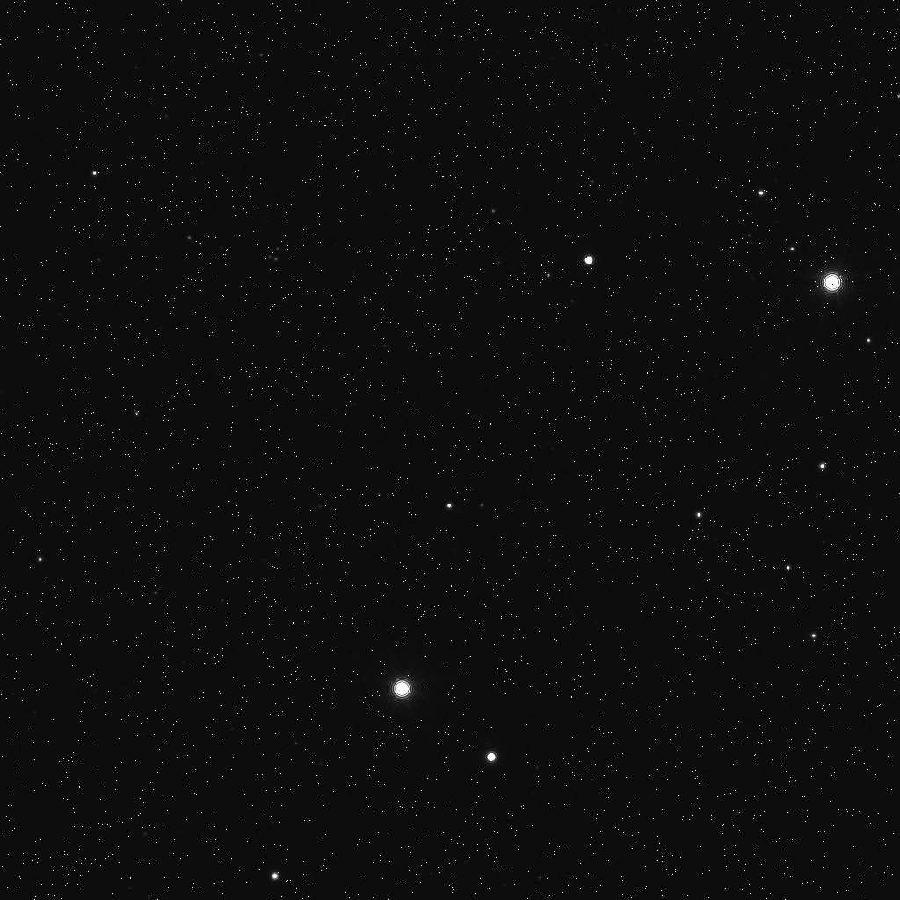
\includegraphics[width=0.23\textwidth]{Figures/Simulated_130_12.pdf} &
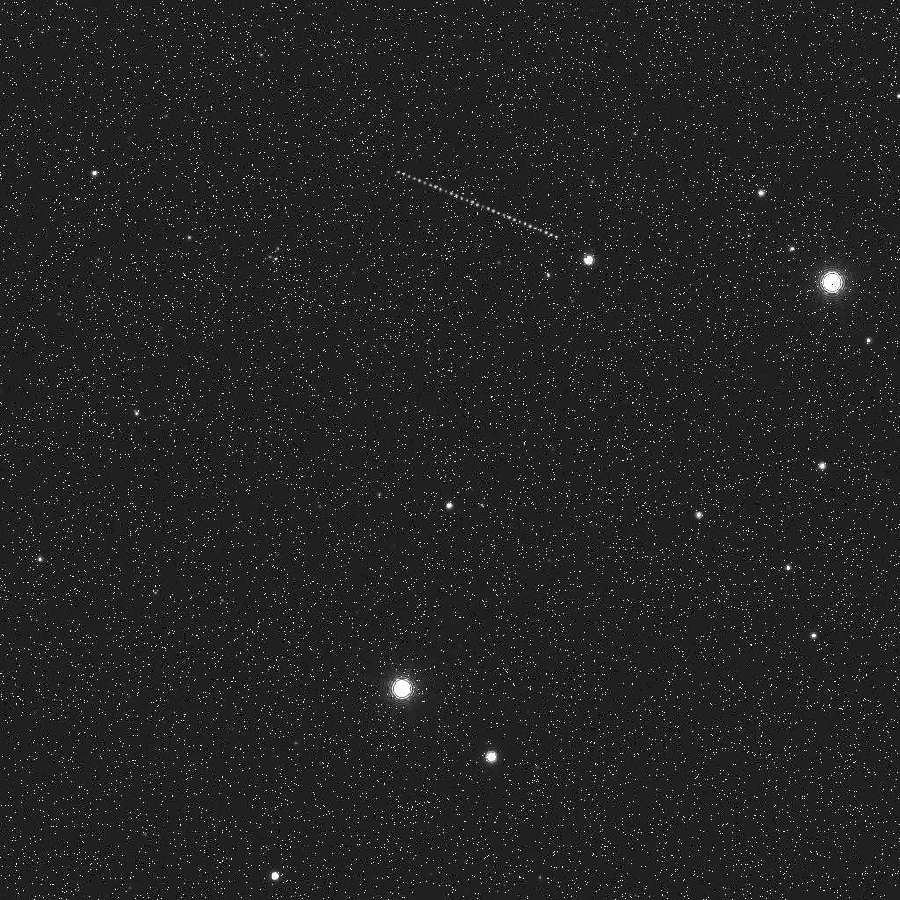
\includegraphics[width=0.23\textwidth]{Figures/TrueTrajectory_130.pdf} 
\end{array}$
\end{center}
\vspace{-0.7cm}
\caption[caption]{Left: An image simulated by RCE. Right: 31 simulated MWIR images super-imposed in order to visualize the trajectory of the asteroid in a single image. The true trajectory can be seen as a faint line towards the top center of the image}
\label{Simulated_Image}
\end{figure}
%
\begin{figure}[h]
\vspace{-0.3cm}
\begin{center}$
\begin{array}{@{\hspace{0.2em}}c@{\hspace{0.2em}}c@{\hspace{0.2em}}}
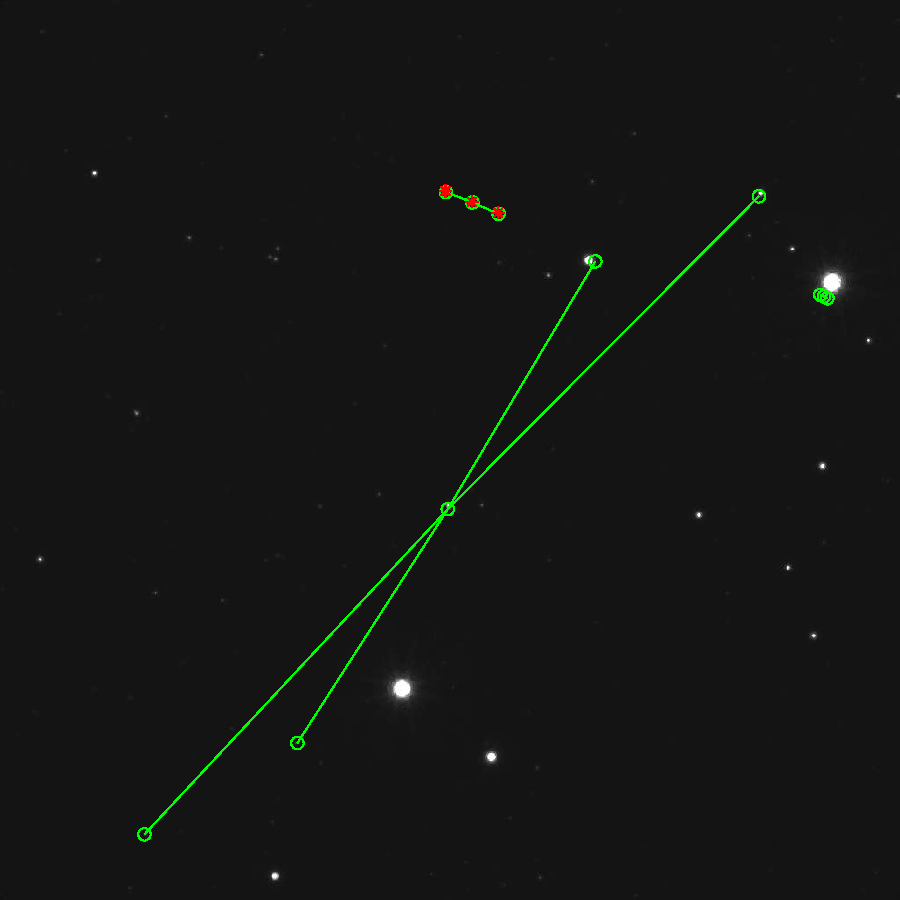
\includegraphics[width=0.23\textwidth]{Figures/Lines_011_016_021.pdf} &
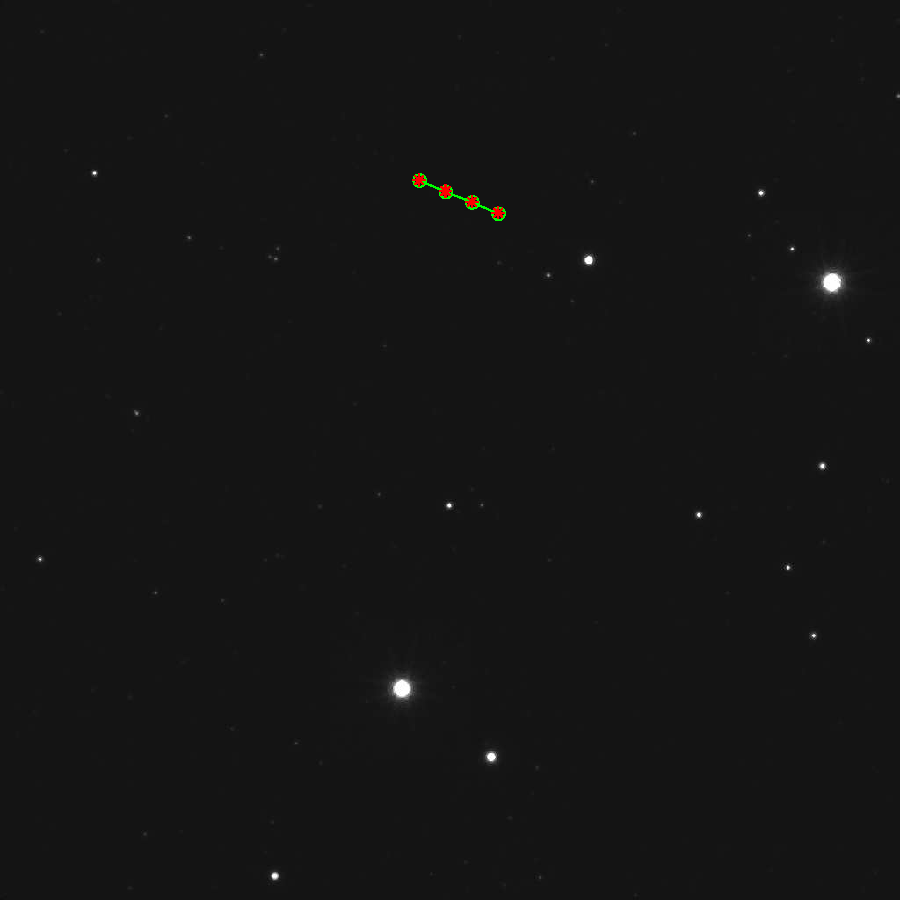
\includegraphics[width=0.23\textwidth]{Figures/Lines_011_016_021_026.pdf} 
\end{array}$
\end{center}
\vspace{-0.7cm}
\caption[caption]{The trajectories found by the pipeline are shown in green. The true location of the asteroid is marked in red.\\\hspace{\textwidth} Left: Trajectory Detection on a simulated triplet.  Right: Trajectory Detection on a quadruplet. Adding one more image to the triplet eliminates the false positives.}
\label{Trajectories_Sim}
\vspace{-0.4cm}
\end{figure}
%

\vspace{-0.4cm}
\begin{figure}[h]
\begin{center}$
\begin{array}{@{\hspace{-0.7em}}c@{\hspace{0.2em}}c@{\hspace{0.2em}}}
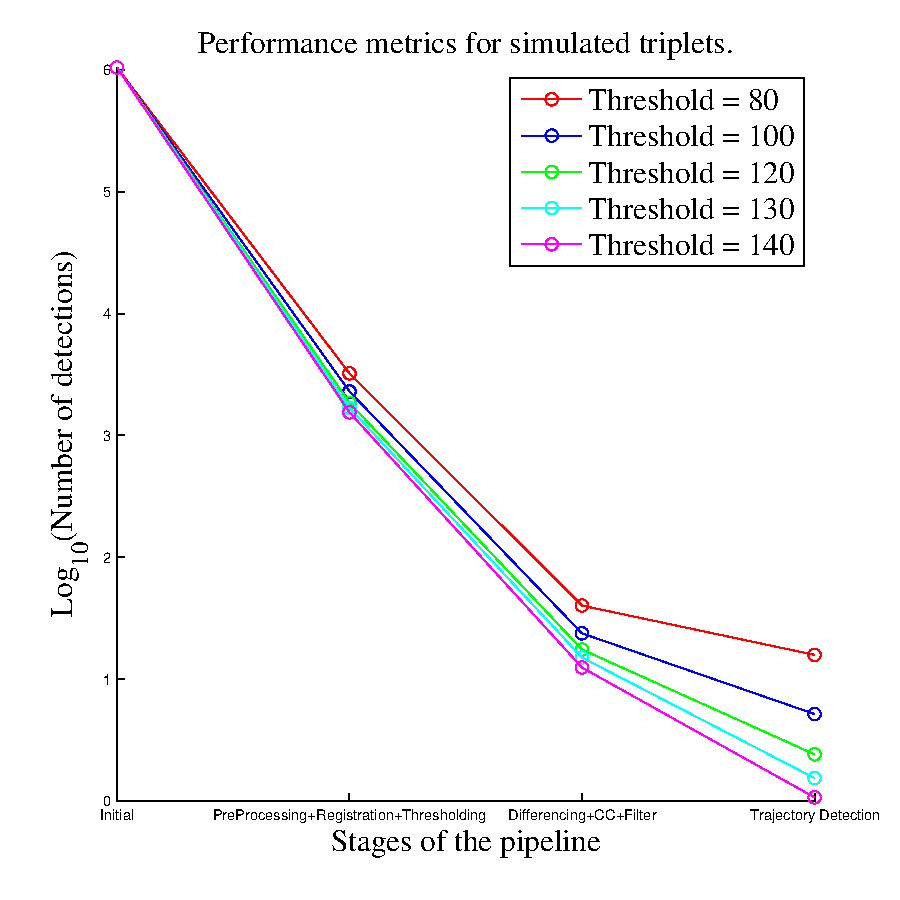
\includegraphics[width=0.25\textwidth]{Figures/Detections_Triplets_Color_f15.pdf} &
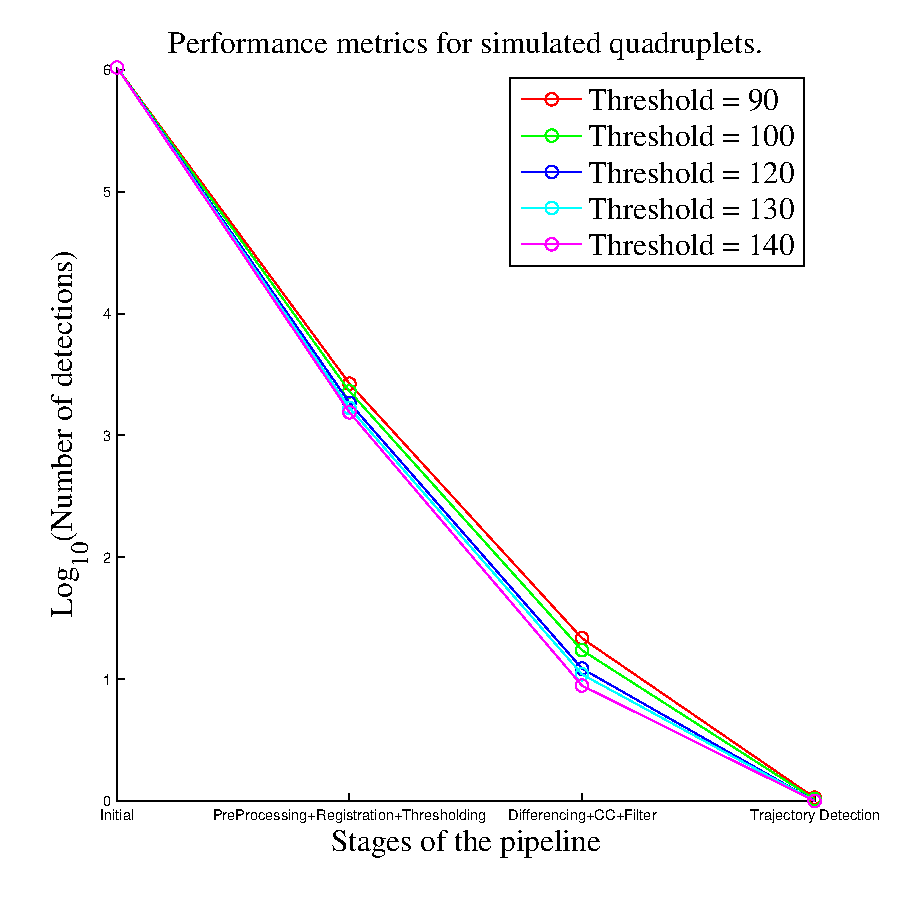
\includegraphics[width=0.25\textwidth]{Figures/Detections_Quad_Color_f15.pdf} 
\end{array}$
\end{center}
\vspace{-0.7cm}
\caption{Left: The number of detections at various stages of the pipeline for triplets of images. Right:  The number of detections at various stages of the pipeline for quadruplets of images.}
\label{num_detect}
\end{figure}
\begin{figure}[h]
\begin{center}$
\begin{array}{@{\hspace{-0.7em}}c@{\hspace{0.2em}}c@{\hspace{0.2em}}}
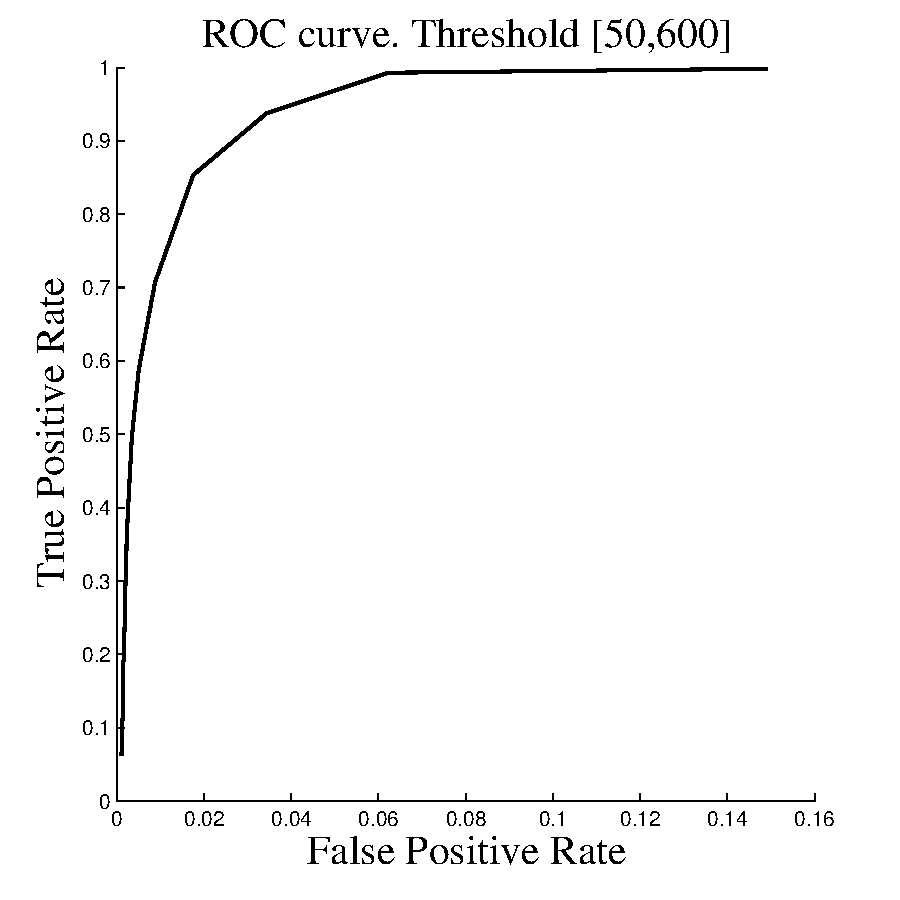
\includegraphics[width=0.25\textwidth]{Figures/ROC_StarAsteroid_130_pchip_f20.pdf} &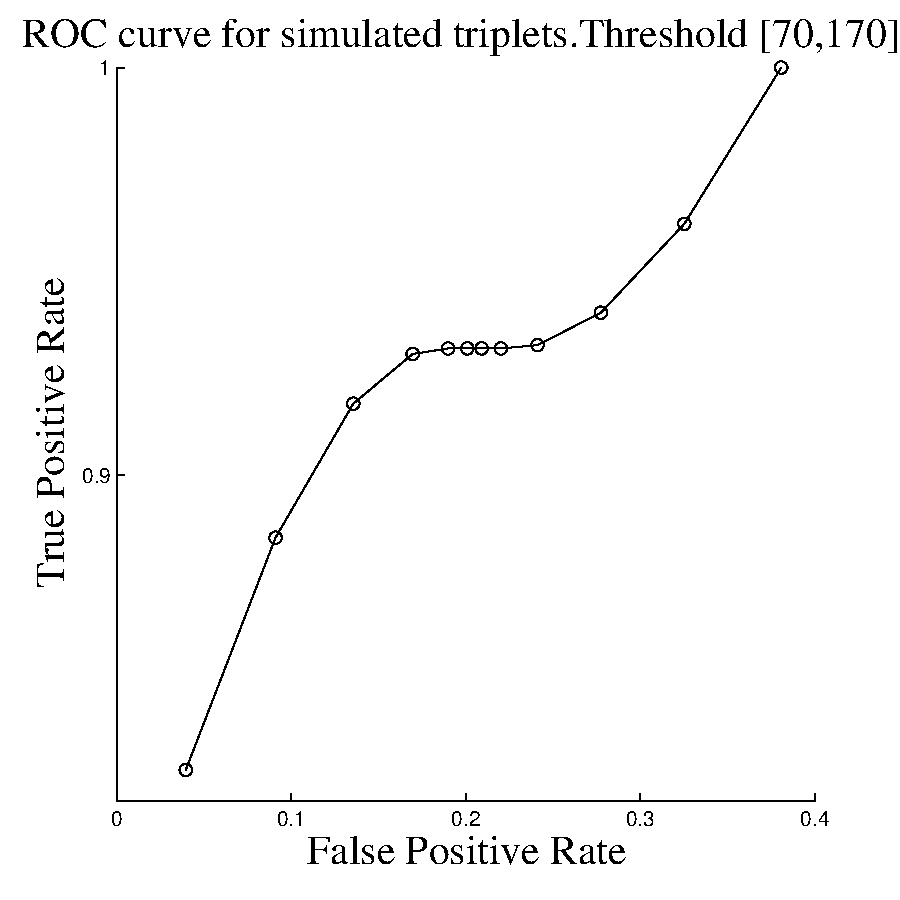
\includegraphics[width=0.25\textwidth]{Figures/ROC_Triplets_130_pchip_f20.pdf} 
\end{array}$
\end{center}
\vspace{-0.7cm}
\caption{Left: ROC curve for the detection of stars and asteroids after the Image thresholding stage of the pipeline. Right:  ROC curve for asteroid detections at the final stage of the pipeline.}
\label{fig:ROC}
\vspace{-0.6cm}
\end{figure} 



\subsection{Simulated Space-Based Imagery}
\label{ssec:simulated}

Using RCE, asteroids are  modeled as spherical blackbody-like emitters, 
%(emissivity is less than 1)
with a cross-sectional area that approximates the sizes of actual asteroids and surface temperatures typical of sun-illuminated asteroids in an Earth-like orbit.  Similar to the way stars are modeled, the radiation emitted is modeled using a form of Planck's equation:

\vspace{-0.3cm}
\begin{equation}
\label{eq:Planck}
B_\lambda(T)= \epsilon	\frac{2hc^2}{\lambda^5} \frac{1}{e^{\frac{hc}{\lambda k_BT}} - 1}
\end{equation}
%\vspace{-0.04cm}
 where $B_\lambda(T)$ is the spectral radiance at a given wavelength $\lambda$ and temperature $T$ %(which in SI units would be $Wm^{-2} m^{-1}$). 
 The value $\epsilon$ is the emissivity of the asteroid, which essentially converts the blackbody spectral radiance into spectral irradiance. The constant, $h$ is the Planck's constant, $c$ is the speed of light, $\lambda$ is wavelength, $k_B$ is the Boltzmann constant, and $T$ is the temperature. 
 
 The asteroids are assumed to have a nominal temperature of 200 K due to solar heating and emissivities in the range from 0.9 to 0.98. 
 %Therefore, their spectral radiance would look like what is shown in Figure \ref{}(TODO: Add this figure? The plot in the year end report does not have the axes labeled.).  For this 200 K blackbody, the peak in the radiance occurs at a wavelength of 14.5 µm.
 The RCE uses stellar data available as part of the Two Micron All Sky Survey (2MASS), a stellar survey that scanned the entire sky in three IR bands (centered at 1.25 \textmu m, 1.65 \textmu m, and 2.17 \textmu m, respectively).  The 2MASS catalog also incorporates data in two visible bands from other surveys. 
 %
 An example of the simulated MWIR image and the ground truth trajectory derived from one set of simulated imagery is shown in Fig. \ref{Simulated_Image}. 
 %In this figure, the simulated images are super-imposed in order to visualize the asteroid trajectory in a single image. 
 %
 Fig. \ref{Trajectories_Sim} shows the final trajectories detected by our algorithm for one triplet and one quadruplet of the simulated MWIR dataset. As is shown in Fig. \ref{Trajectories_Sim}, using trajectory verification on a greater number of images in the sequence allows us to quickly disambiguate and reject false trajectories. In this case this trend is readily apparent when going from a triplet to a quadruplet of images.
%

We characterize the algorithm with regard to detections at each of the following three successive stages: the initial detection of objects, the detection of moving objects and the detection of trajectories.
In Fig.~\ref{num_detect}, we plot the number of detected objects at each step of the pipeline for each selected threshold value. We can verify that the number of detections monotonically decreases when the threshold increases. Note that we have found that this not always the case, especially since a higher number of detections at the thresholding stage may induce more cancellations at the logical differencing. Additionally, we note in the right plot in Fig.~\ref{num_detect} that the use of quadruplets allows for a single trajectory to be found irrespective of the value of the threshold used (and hence the number of detections found at the first stage), echoing the results displayed in Fig.~\ref{Trajectories_Sim}.
%
Last, we show the Receiver Operating Characteristic (ROC) for simulated space-based imagery in Fig.~\ref{fig:ROC}.  
%
%Results for each step of the pipeline are shown:
% Image Registration in Figure~\ref{}. Logical differencing in Figure~\ref{}. (See Figure ~\ref{} for trajectory detection on an example image triplet).    As is shown in Figure~\ref{}, using trajectory verification on a greater number of images in the sequence allows us to quickly disambiguate and reject false trajectories (in this case this trend is readily apparent when going from a triplet to a quadruplet of images).

\subsection{Real Imagery}

\subsubsection{NEAT}
Near Earth Asteroid Tracking (NEAT)~\cite{neat2014} is an earth-based program run by NASA from 1995-2007 to discover NEOs.
Fig. \ref{IPP_NEAT_Layout1} and Fig. \ref{fig:IPP_NEAT_Trajectory} show the results at all stages of the pipeline for one triplet of images of the 2002-CY46 asteroid obtained from the NEAT system archive. 
%The following figures show the results at all stages of the pipeline for one triplet of images of the 2002-CY46 asteroid obtained from the NEAT \cite{neat2014} survey. 
 
%\begin{figure*}
%\minipage{0.33\textwidth}
%  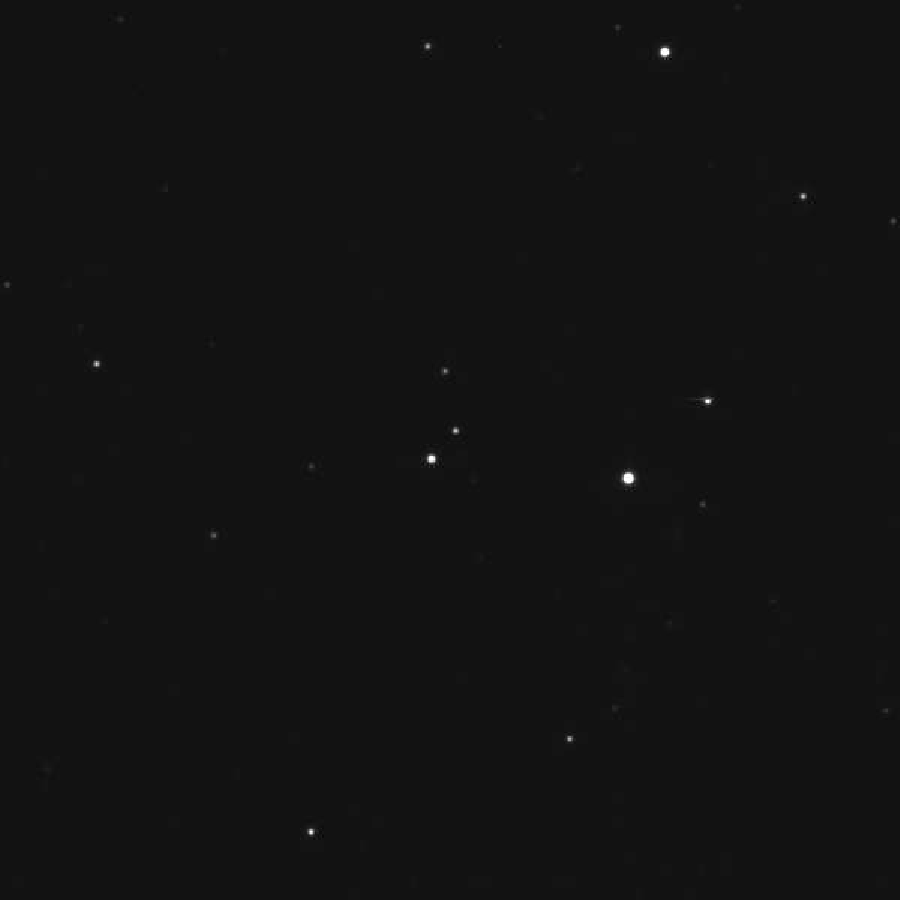
\includegraphics[width=\linewidth]{Figures/NEAT1.pdf}
%\endminipage\hfill
%\minipage{0.33\textwidth}
%  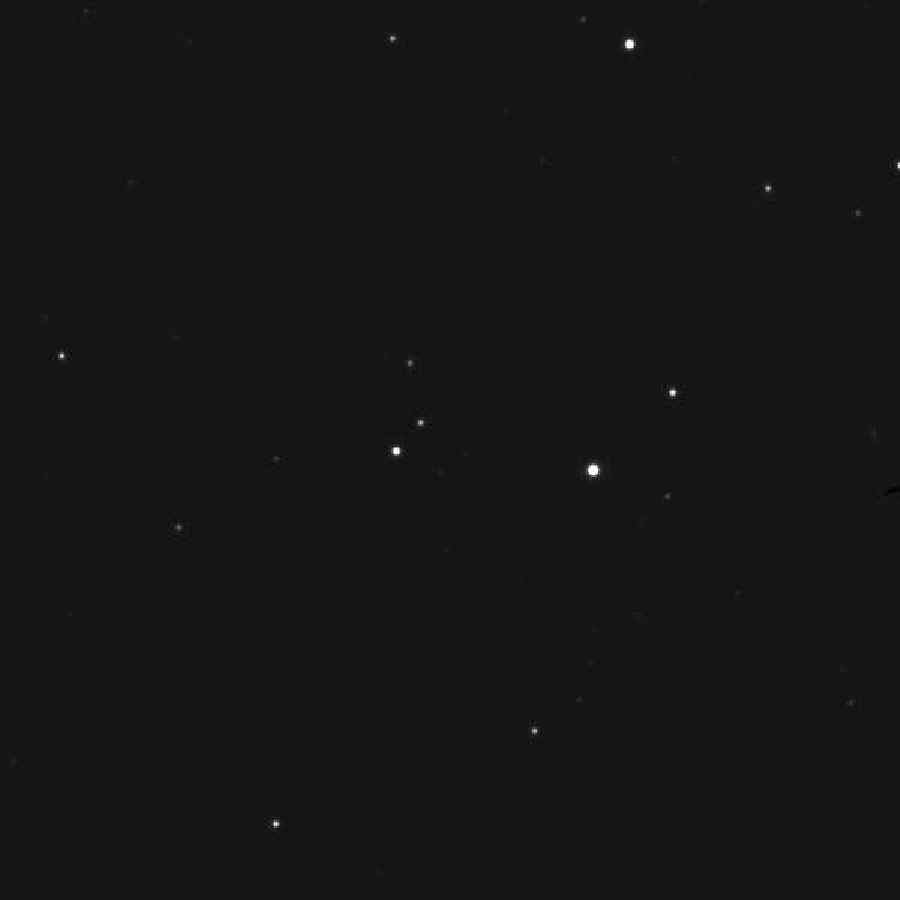
\includegraphics[width=\linewidth]{Figures/NEAT2.pdf}
%\endminipage\hfill
%\minipage{0.33\textwidth}
%  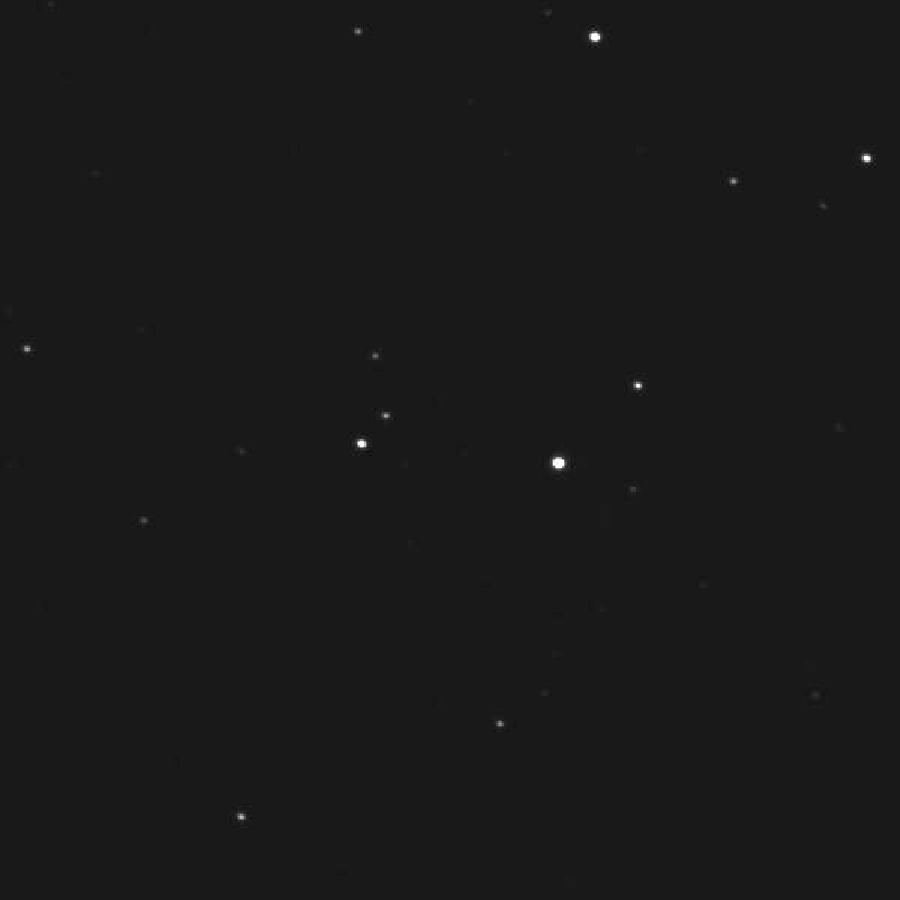
\includegraphics[width=\linewidth]{Figures/NEAT3.pdf}
%\endminipage
%\caption{2002 CY46 Triplet Near Earth Asteroid Tracking (NEAT) system archive}
%\label{fig:NEAT_Images}
%\end{figure*}
\vspace{-0.2cm}
\newcommand{\imgWidth}{0.15\textwidth}
\begin{figure}[h]
\begin{center}$
\begin{array}{@{\hspace{0.2em}}c@{\hspace{0.3em}}c@{\hspace{0.3em}}c}
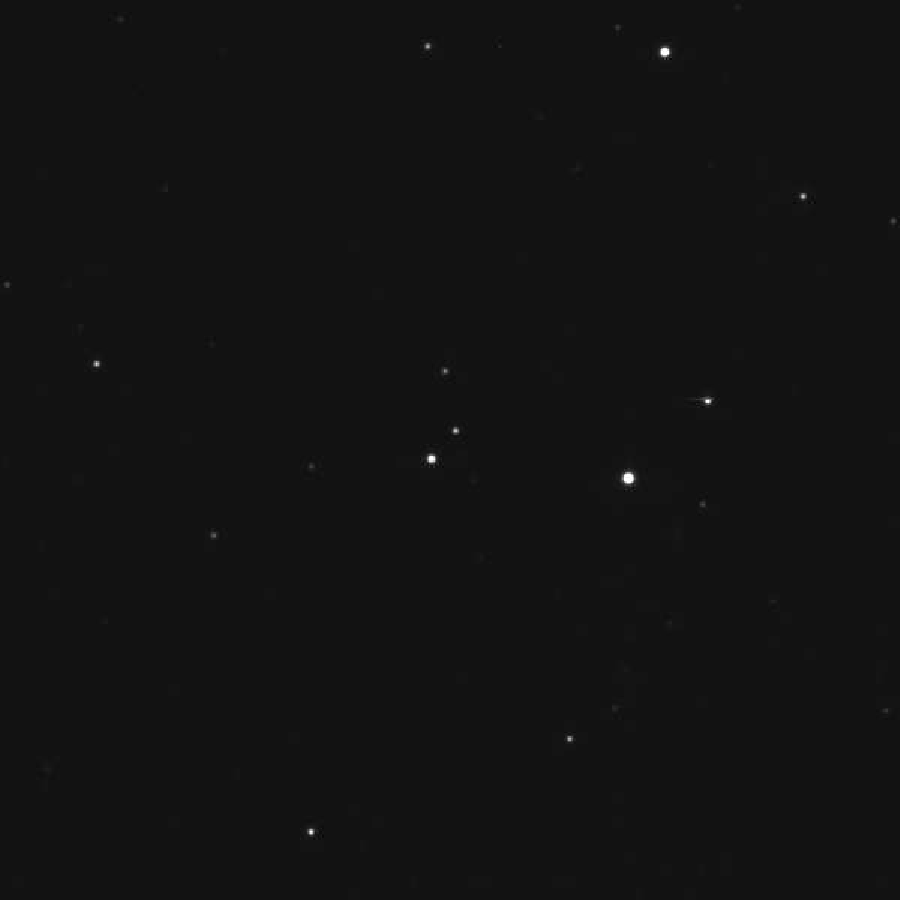
\includegraphics[width=\imgWidth]{Figures/NEAT1.pdf} &
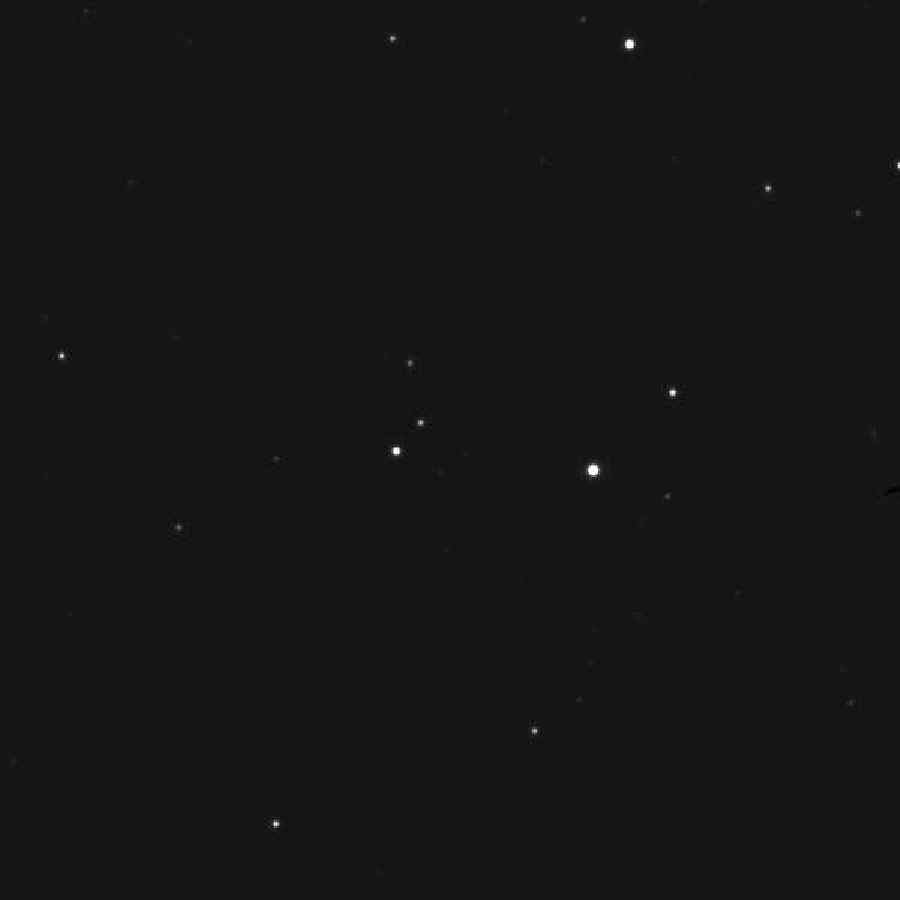
\includegraphics[width=\imgWidth]{Figures/NEAT2.pdf} &
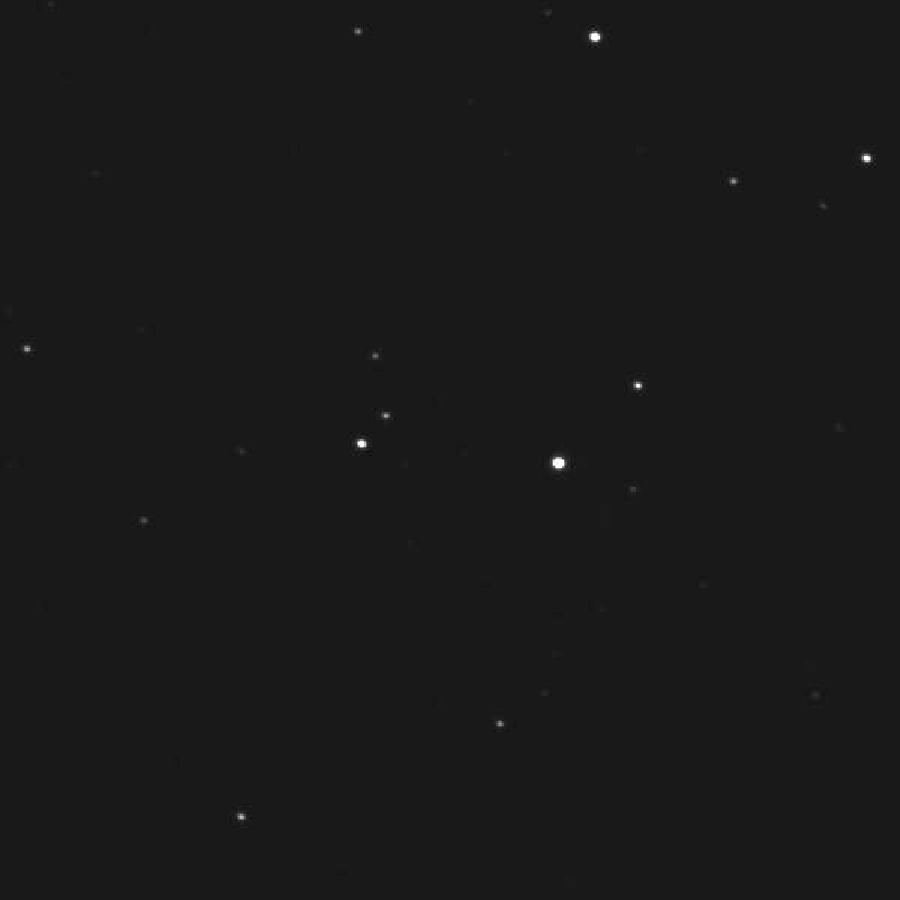
\includegraphics[width=\imgWidth]{Figures/NEAT3.pdf} \\
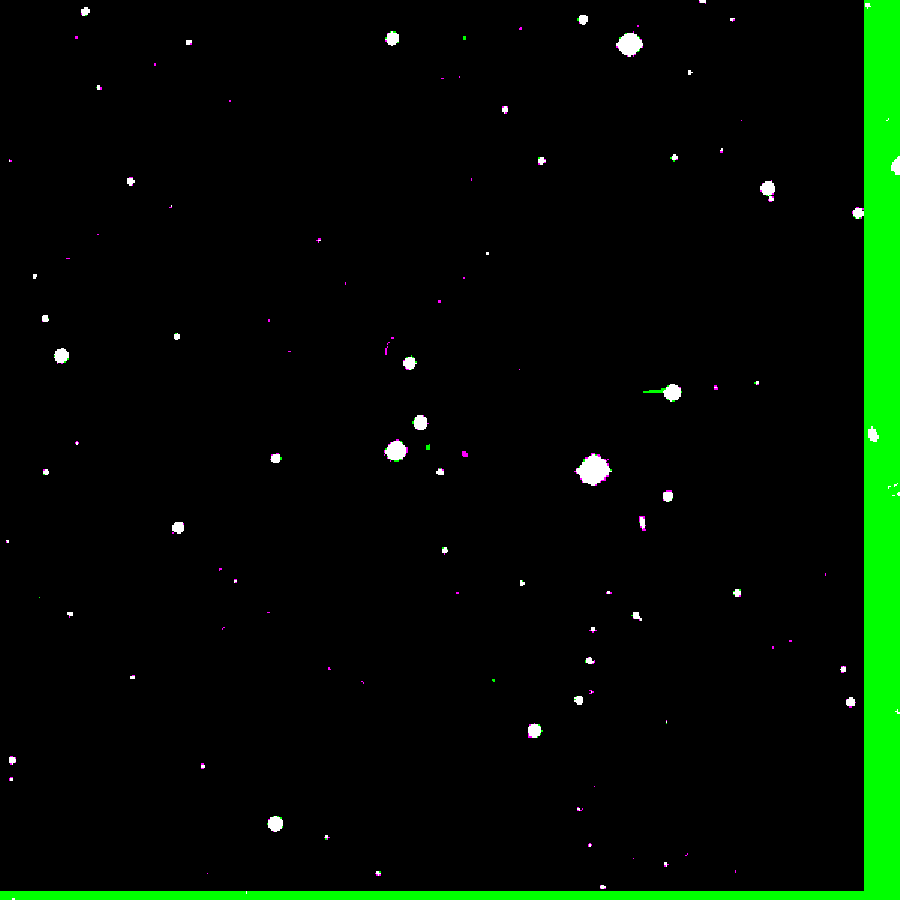
\includegraphics[width=\imgWidth]{Figures/NEATImageReg12.pdf} &
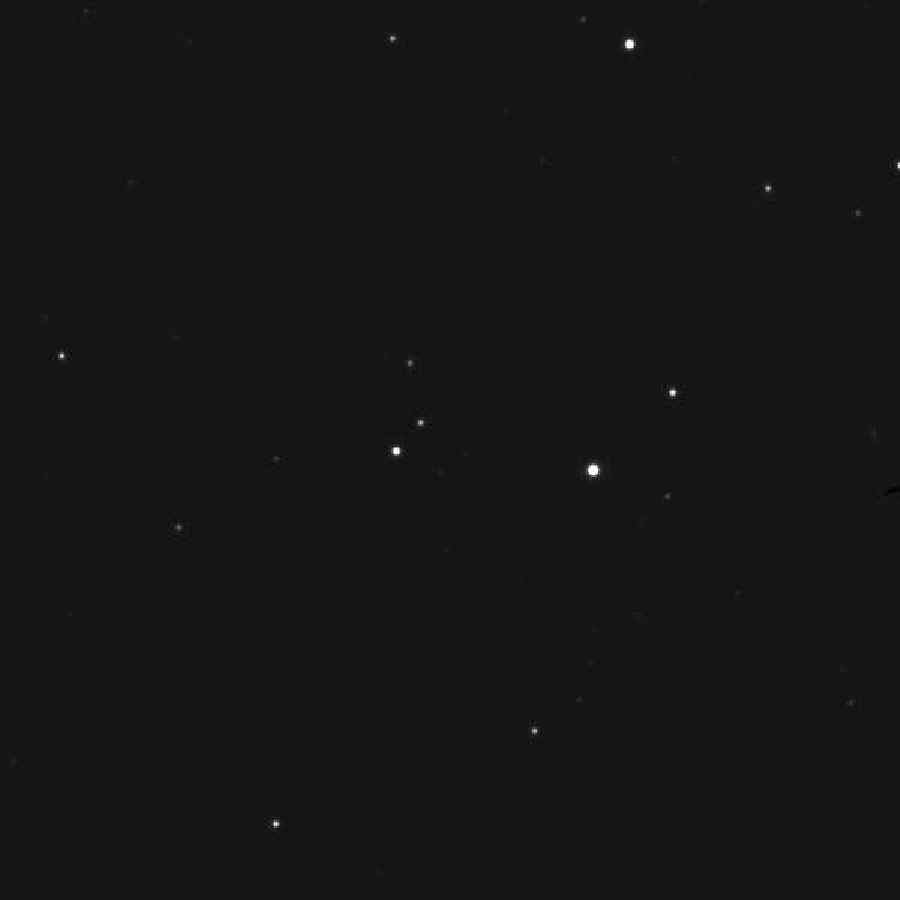
\includegraphics[width=\imgWidth]{Figures/NEAT2.pdf} &
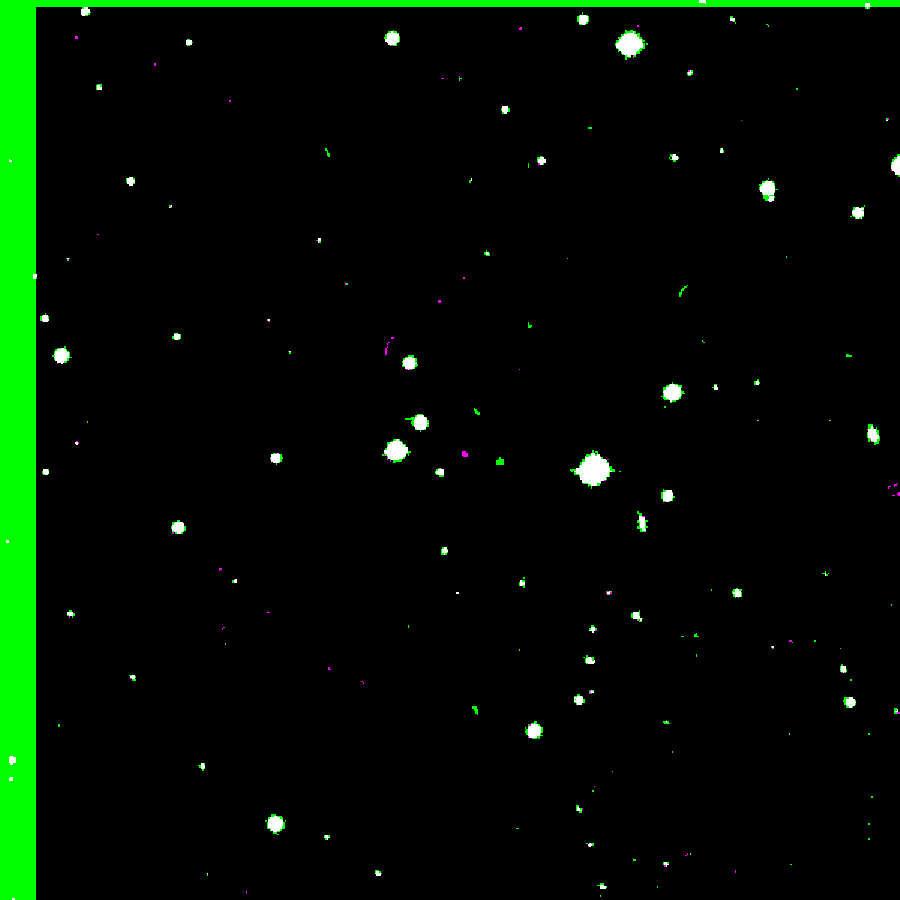
\includegraphics[width=\imgWidth]{Figures/NEATImageReg32.pdf} \\
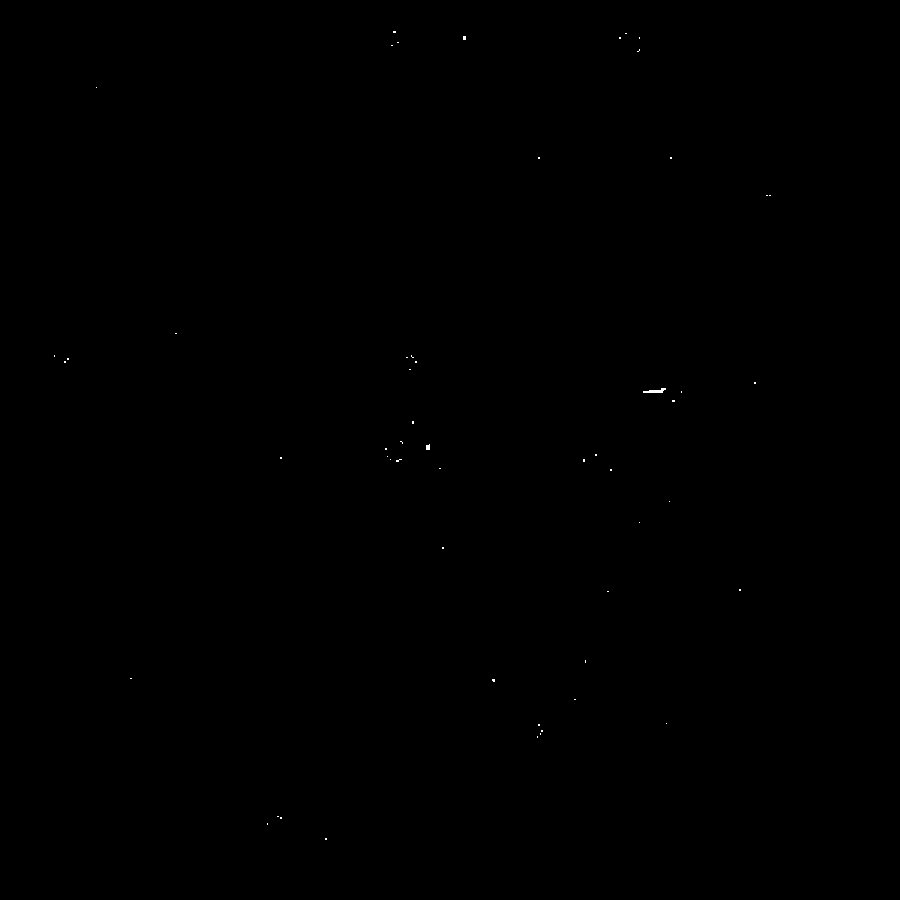
\includegraphics[width=\imgWidth]{Figures/NEATImageDiff1.pdf} &
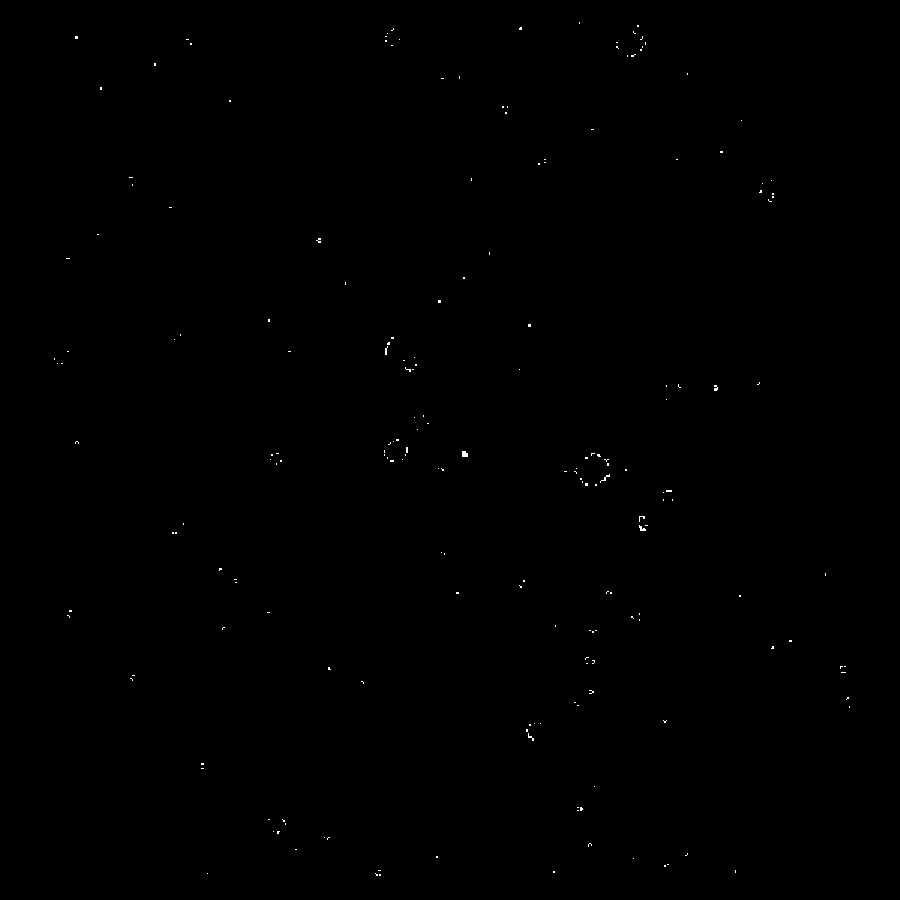
\includegraphics[width=\imgWidth]{Figures/NEATImageDiff2.pdf} &
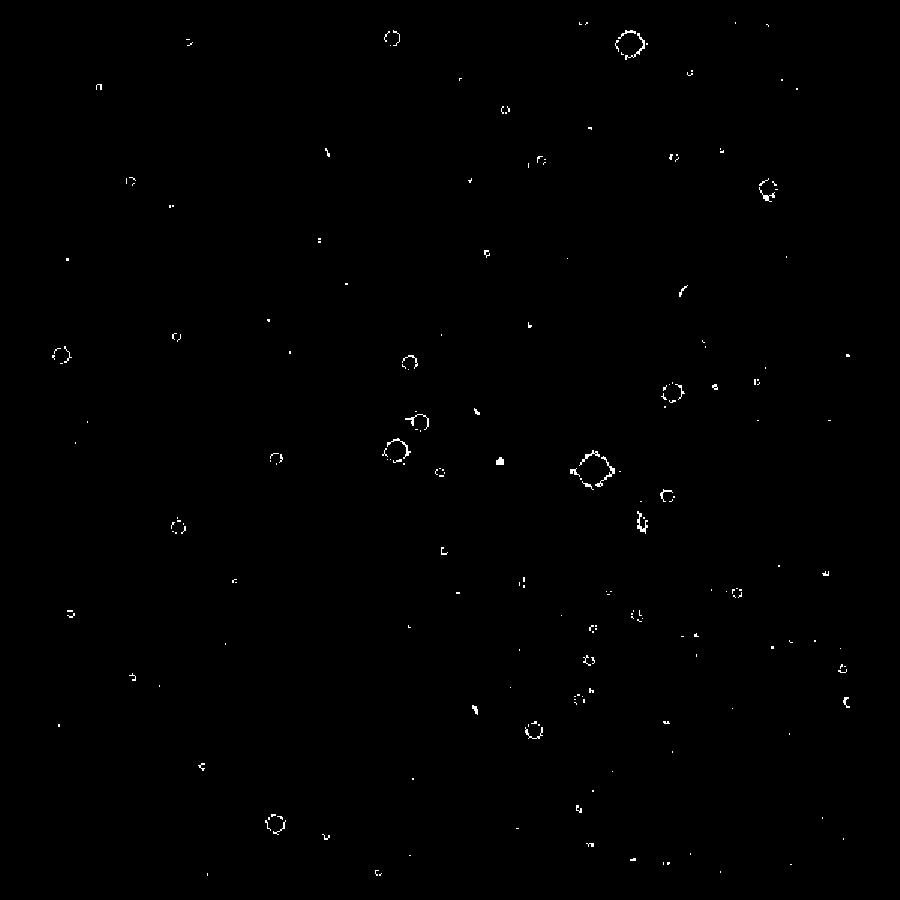
\includegraphics[width=\imgWidth]{Figures/NEATImageDiff3.pdf} \\
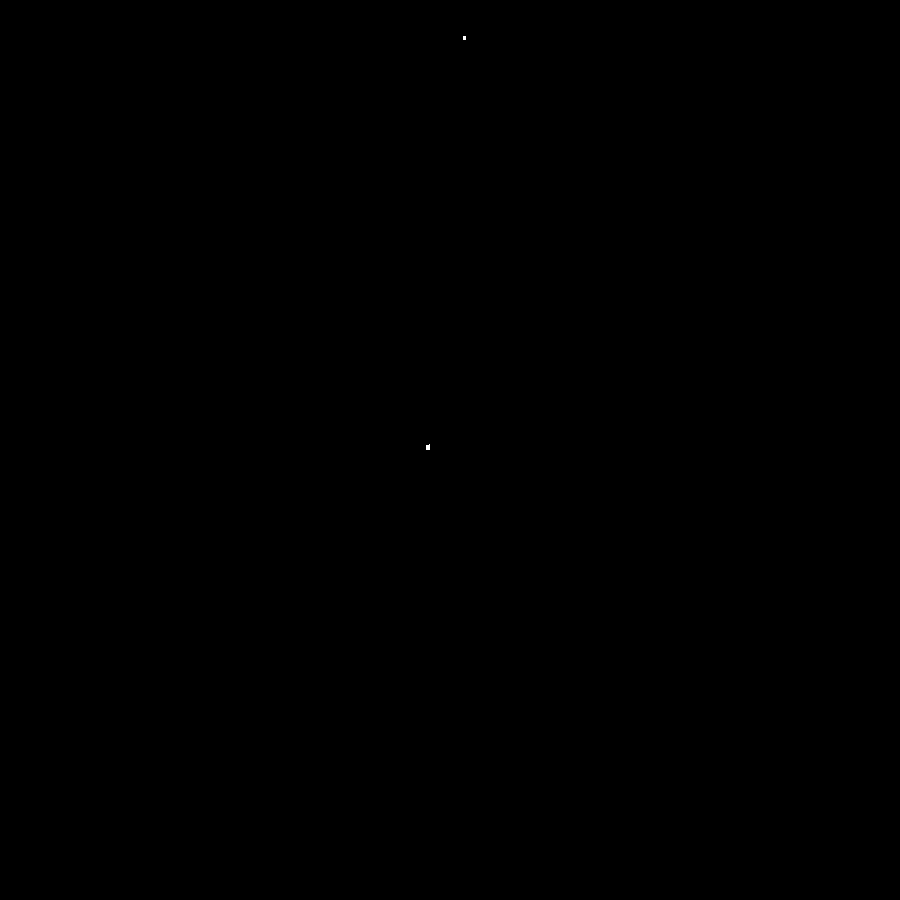
\includegraphics[width=\imgWidth]{Figures/NEATFilteredCentroids1.pdf} &
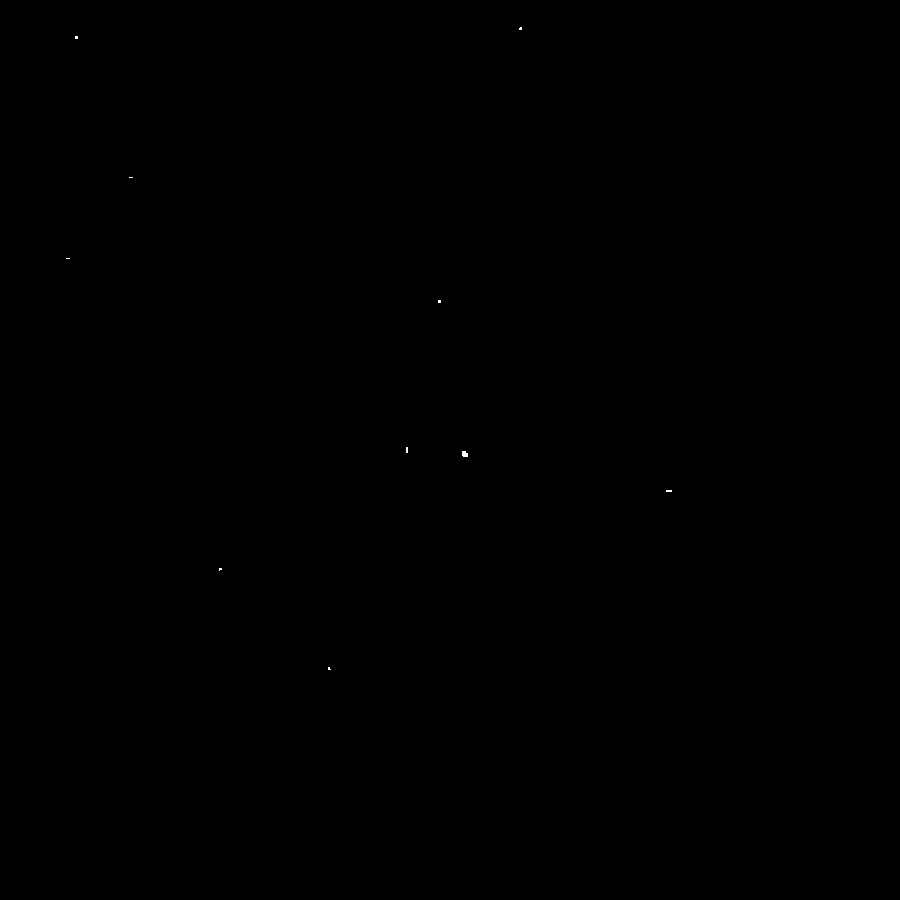
\includegraphics[width=\imgWidth]{Figures/NEATFilteredCentroids2.pdf} &
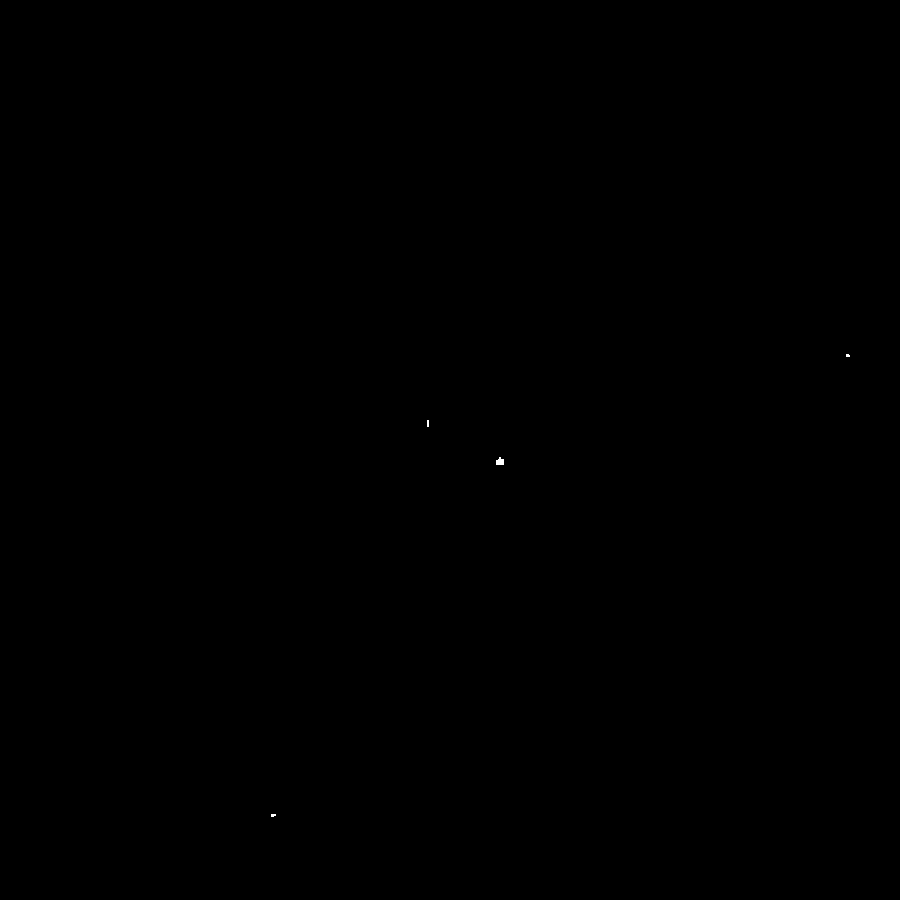
\includegraphics[width=\imgWidth]{Figures/NEATFilteredCentroids3.pdf}
\end{array}$
\end{center}
\vspace{-0.7cm}
\caption[caption]{Image Processing Pipeline results shown on 2002 NEAT data. 
(row 1):  input image triplet (CY46) taken approx. 10 minutes apart. 
(row 2): Image Registration. Left: Image-1 registered to Image-2. Right: Image-3 registered to Image-2. 
%\\\hspace{\textwidth} 
(row 3): Image Differencing: Artifacts such as crater-like formations are seen in the difference images above. This is the result of some celestial bodies being over-exposed.) 
%\\\hspace{\textwidth} 
(row 4): Image Differencing: Filtered centroids shown in each image of the sequence.)}
\label{IPP_NEAT_Layout1}
\end{figure}

\begin{figure}[!]
%\minipage{0.40\textwidth}
%  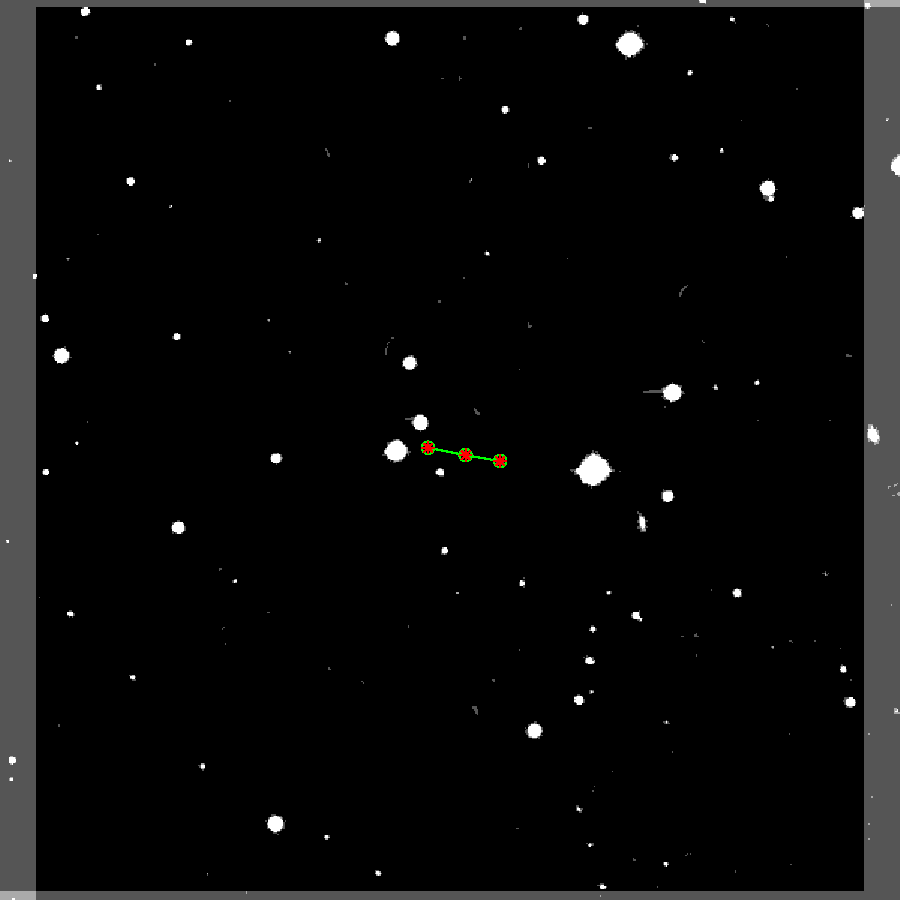
\includegraphics[width=\linewidth]{Figures/NEATLines_LogicalImg.pdf}
%\endminipage\hfill
\vspace{-0.25cm}
\begin{center}
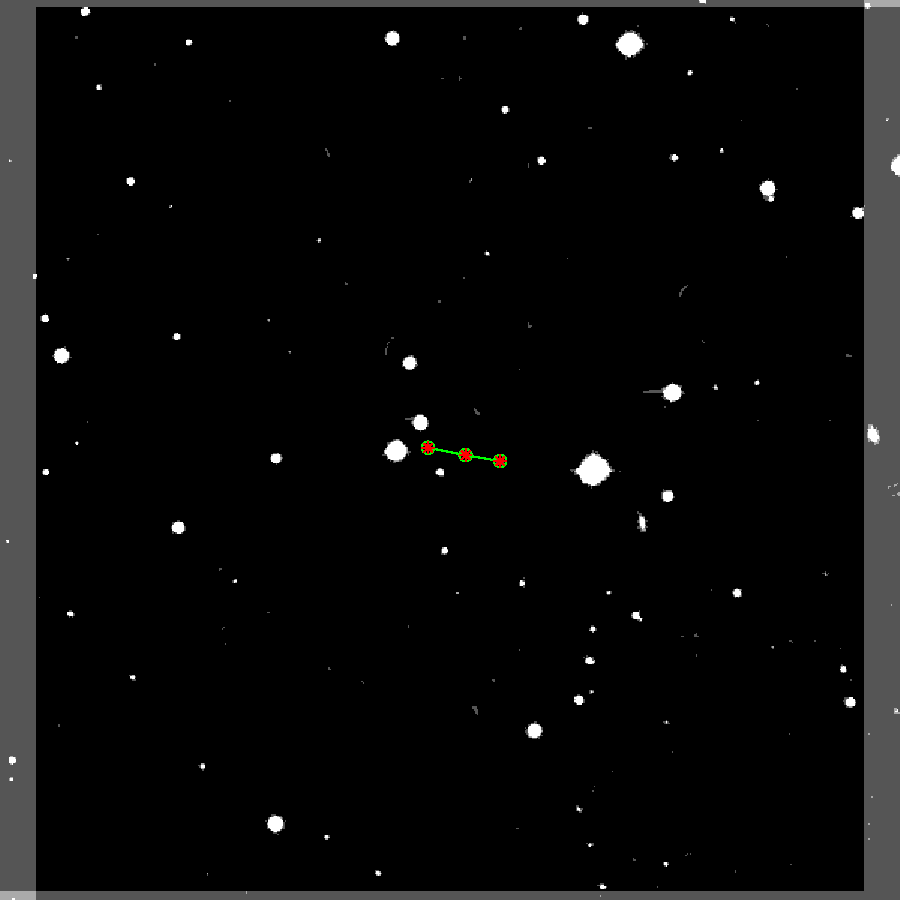
\includegraphics[width=0.3\textwidth]{Figures/NEATLines_LogicalImg.pdf}
\end{center}
\vspace{-0.7cm}
\caption{Trajectory Detection for the NEAT CY46 Triplet. Asteroid trajectory detected is shown in green. True location is in red. 3 Images of the triplet are super-imposed here after registration and thresholding for ease of visualization.}
\label{fig:IPP_NEAT_Trajectory}
\vspace{-0.3cm}
\end{figure}

\begin{figure}[h]
\vspace{-0.1cm}
\begin{center}
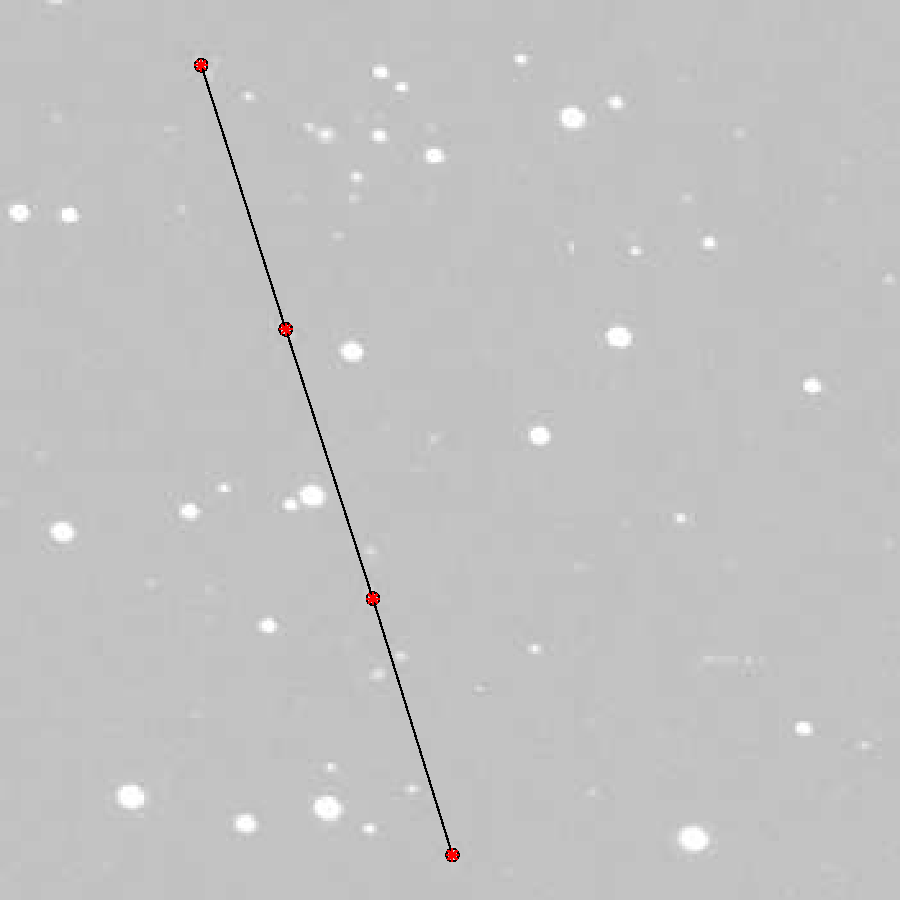
\includegraphics[width=0.3\textwidth]{Figures/CSS_Quad_Black_Lines.pdf} 
\end{center}
\vspace{-0.7cm}
\caption[caption]{Image Processing results shown on Catalina Sky Survey data.}
%\\\hspace{\textwidth} 
\label{IPP_Catalina_Layout1}
\end{figure}

\begin{figure}[h]
\begin{center}$
\begin{array}{@{\hspace{-0.7em}}c@{\hspace{0.2em}}c@{\hspace{0.2em}}}
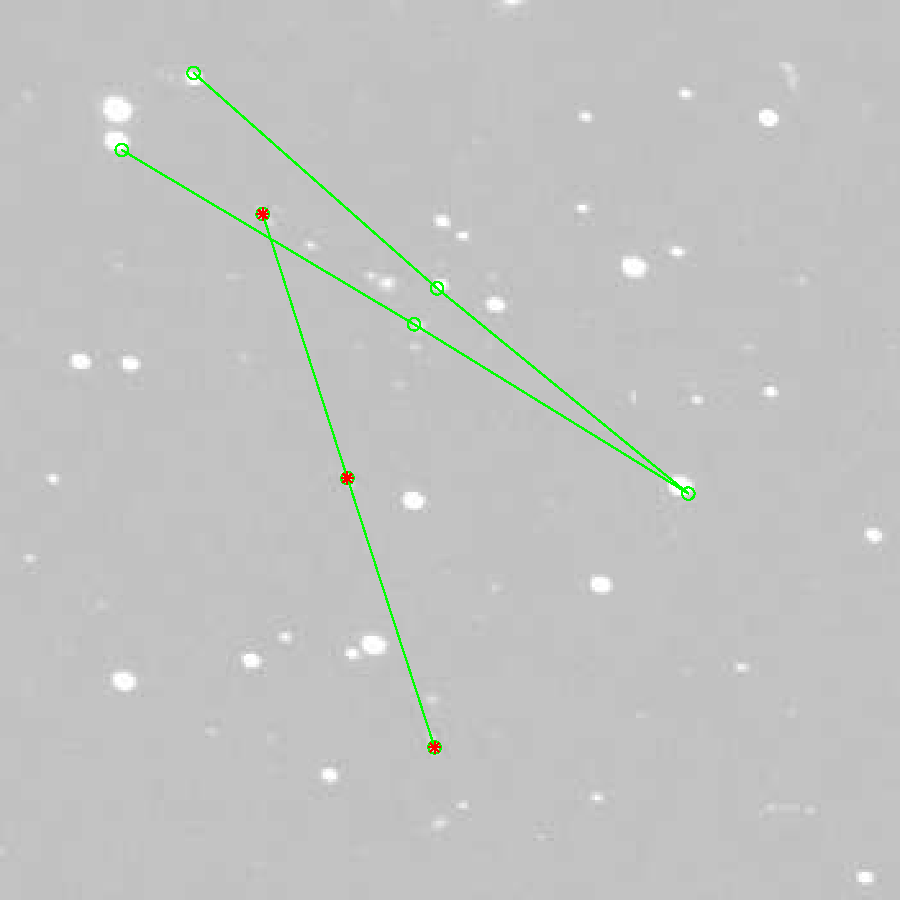
\includegraphics[width=0.25\textwidth]{Figures/CSS_Triplet_Lines.pdf} &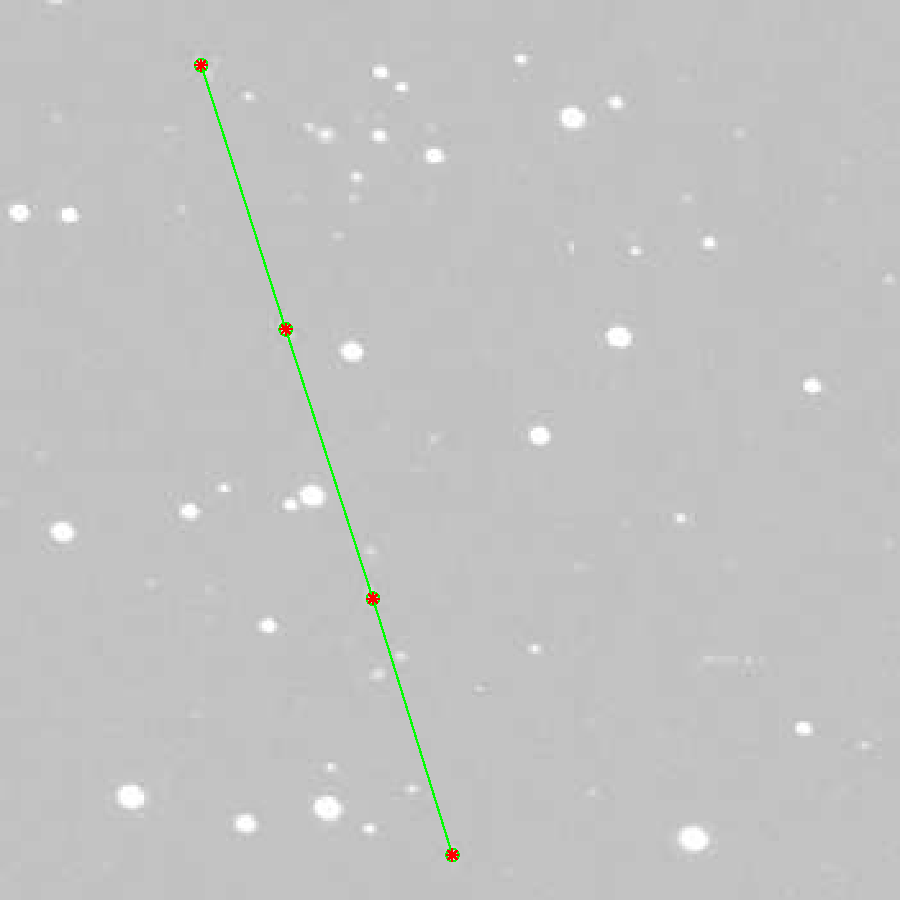
\includegraphics[width=0.25\textwidth]{Figures/CSS_Quad_Lines.pdf} 
\end{array}$
\end{center}
\vspace{-0.7cm}
\caption{Image Processing results shown on Catalina Sky Survey data.}
\label{IPP_Catalina_Layout2}
\vspace{-0.6cm}
\end{figure} 

%
%\begin{figure}[t]
%\vspace{-0.7cm}
%\begin{center}$
%\begin{array}{@{\hspace{0.2em}}c@{\hspace{0.3em}}c@{\hspace{0.3em}}c}
%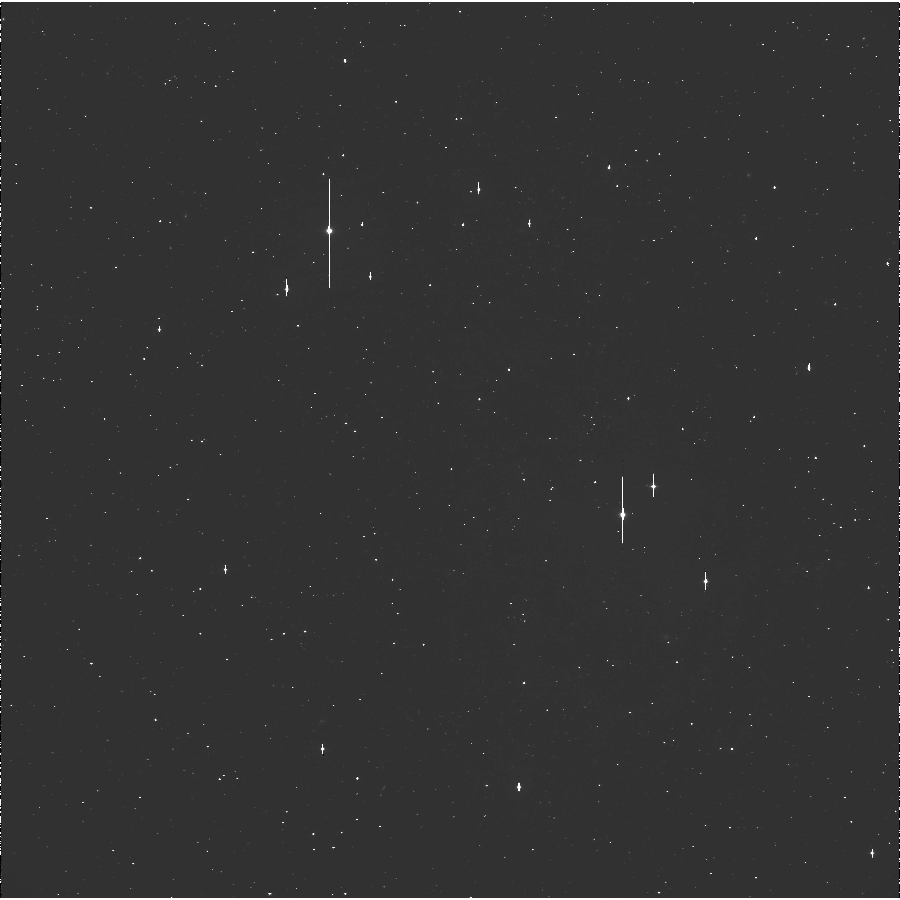
\includegraphics[width=\imgWidth]{Figures/CSS_100_5000_1.pdf} &
%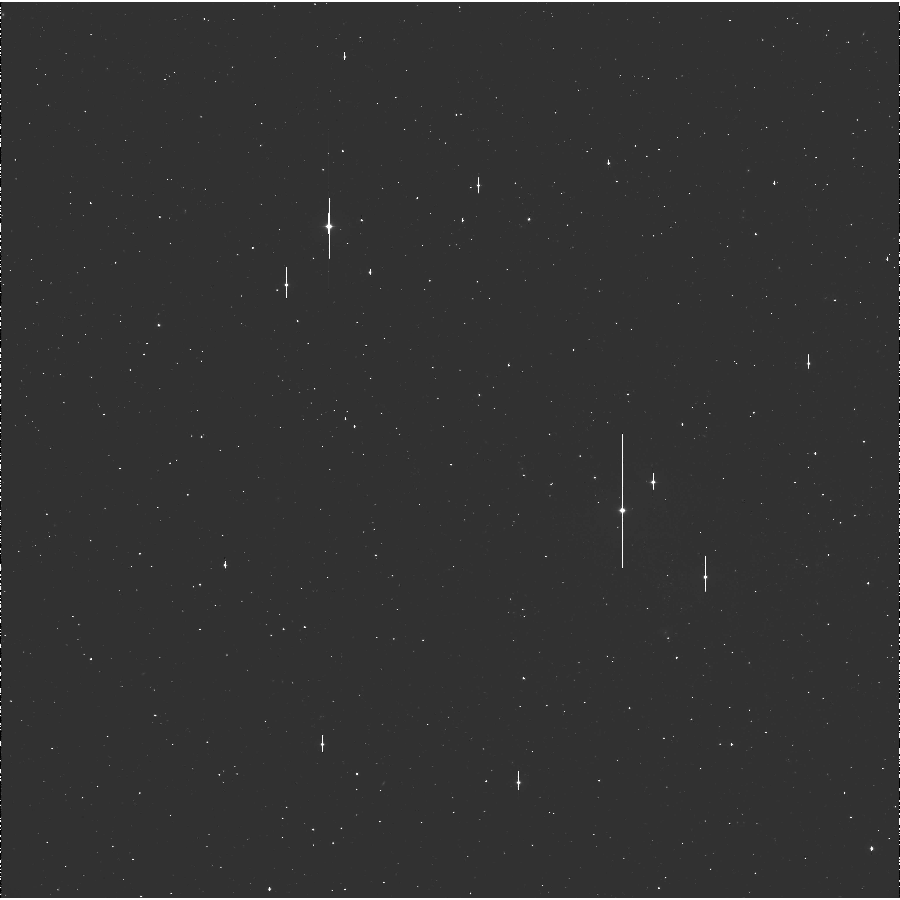
\includegraphics[width=\imgWidth]{Figures/CSS_100_5000_2.pdf} &
%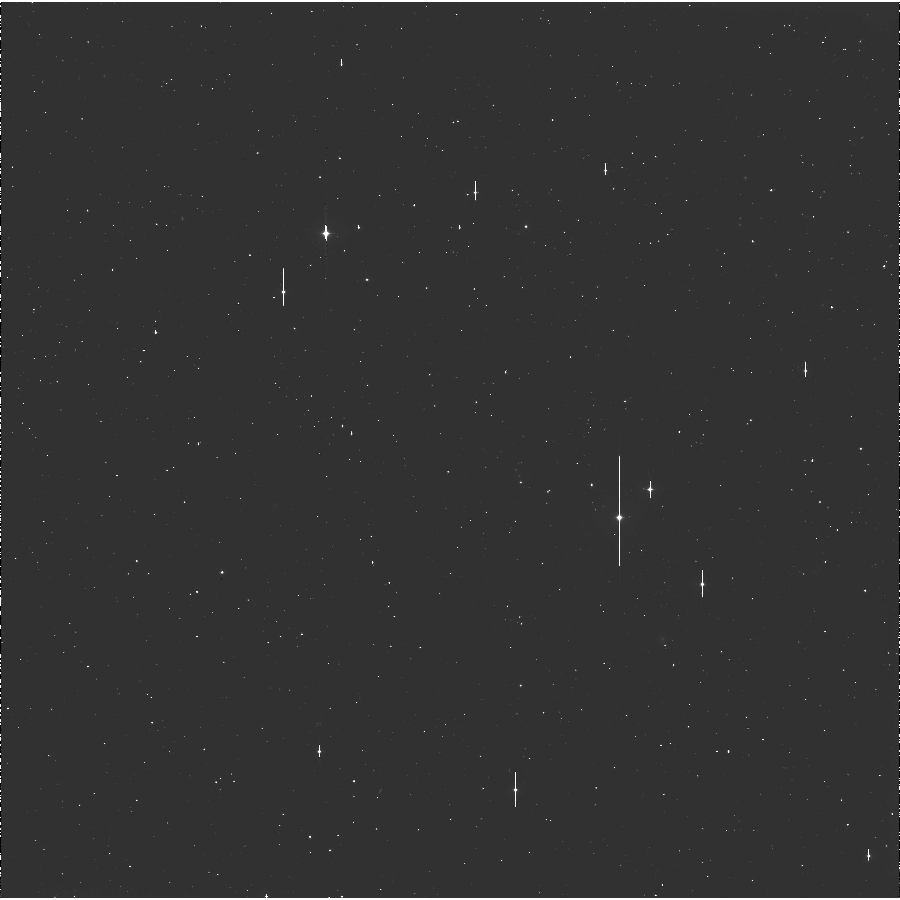
\includegraphics[width=\imgWidth]{Figures/CSS_100_5000_3.pdf} \\
%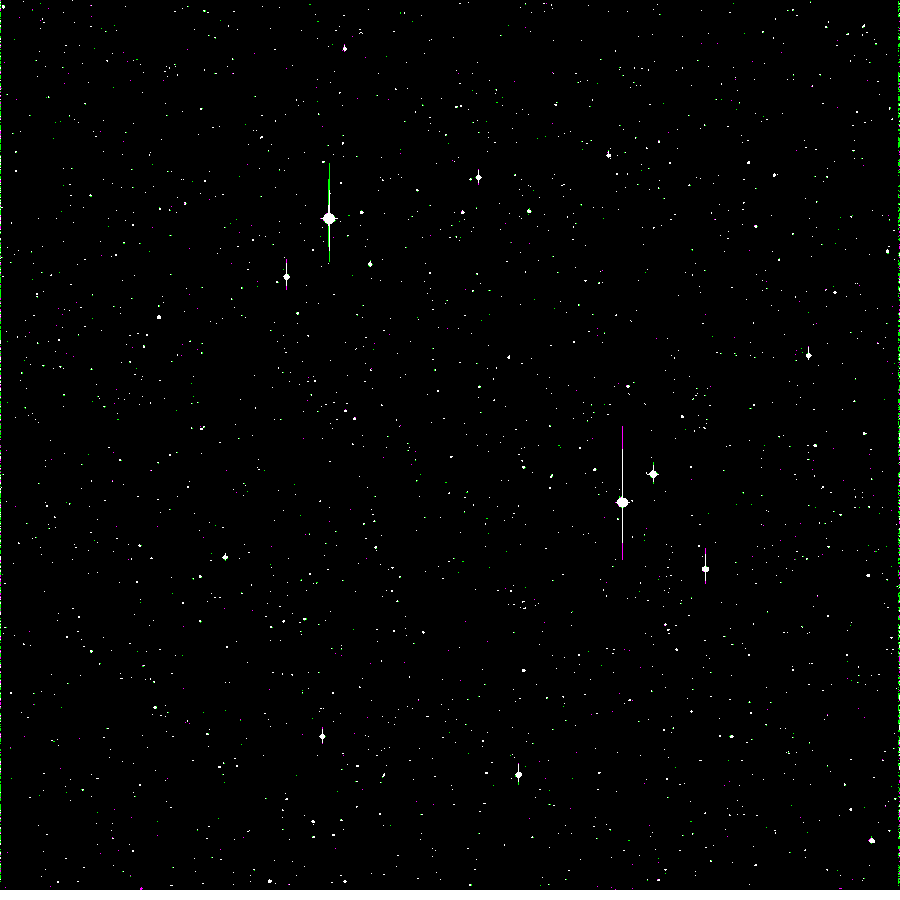
\includegraphics[width=\imgWidth]{Figures/ImageReg12_CSS.pdf} &
%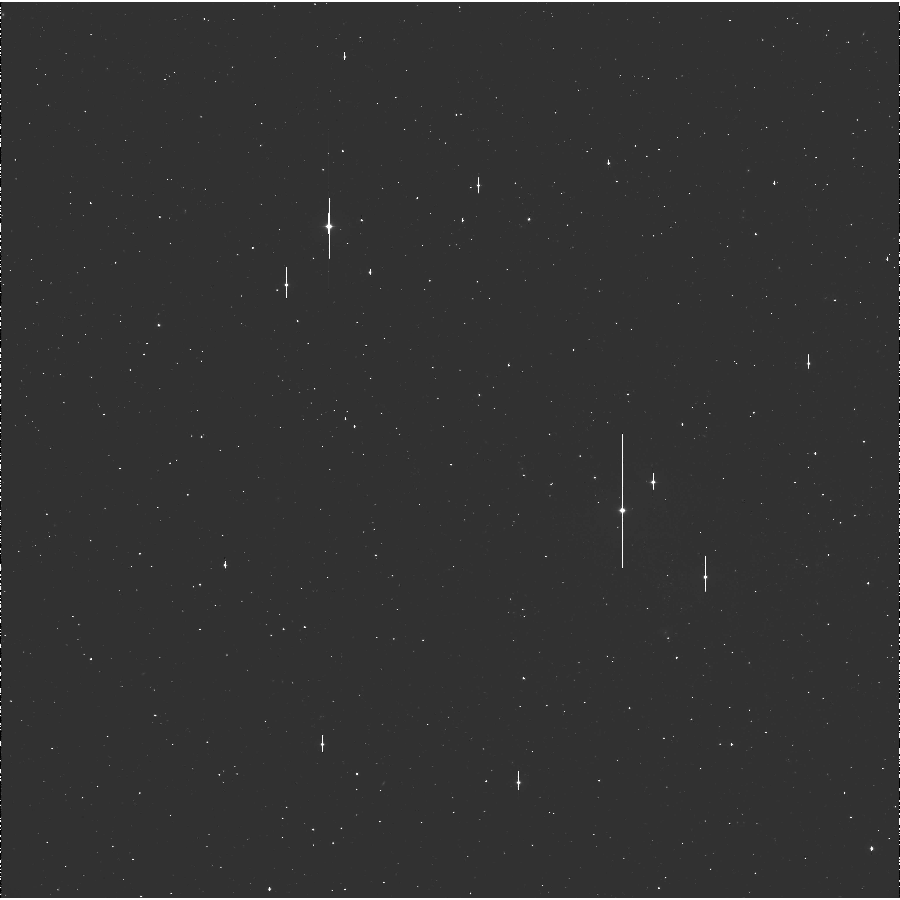
\includegraphics[width=\imgWidth]{Figures/CSS_100_5000_2.pdf} &
%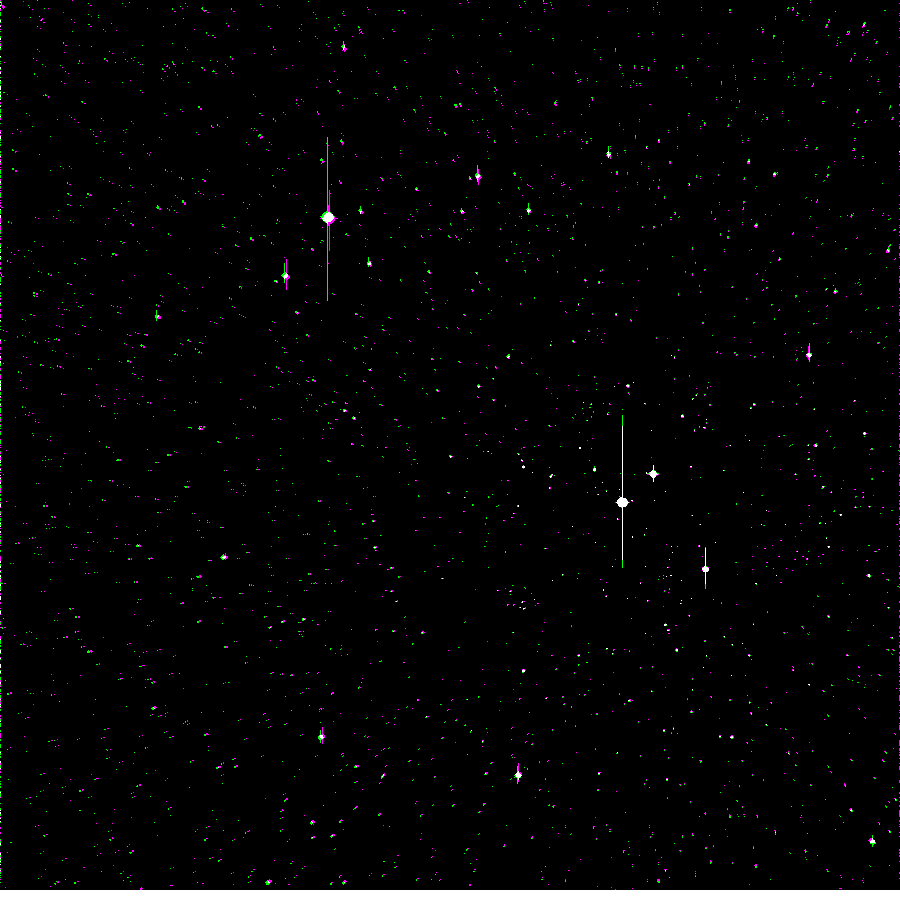
\includegraphics[width=\imgWidth]{Figures/ImageReg32_CSS.pdf} \\
%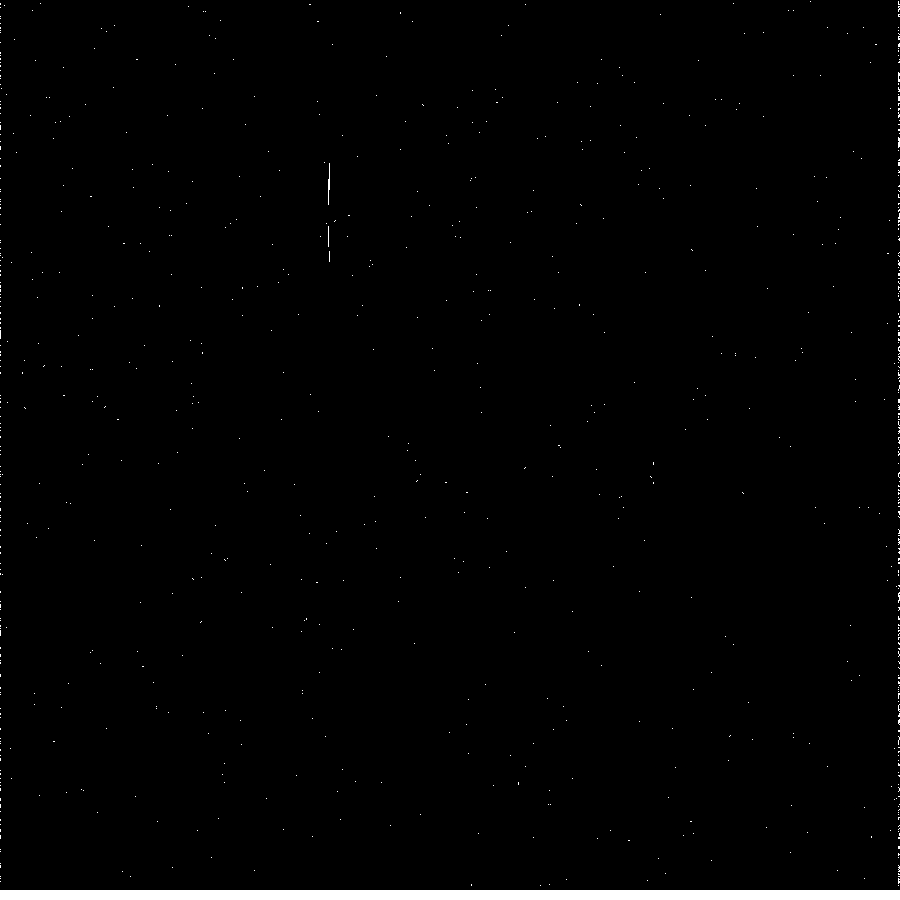
\includegraphics[width=\imgWidth]{Figures/ImageDiff_CSS1.pdf} &
%
\includegraphics[width=\imgWidth]{Figures/ImageDiff_CSS2.pdf} &
%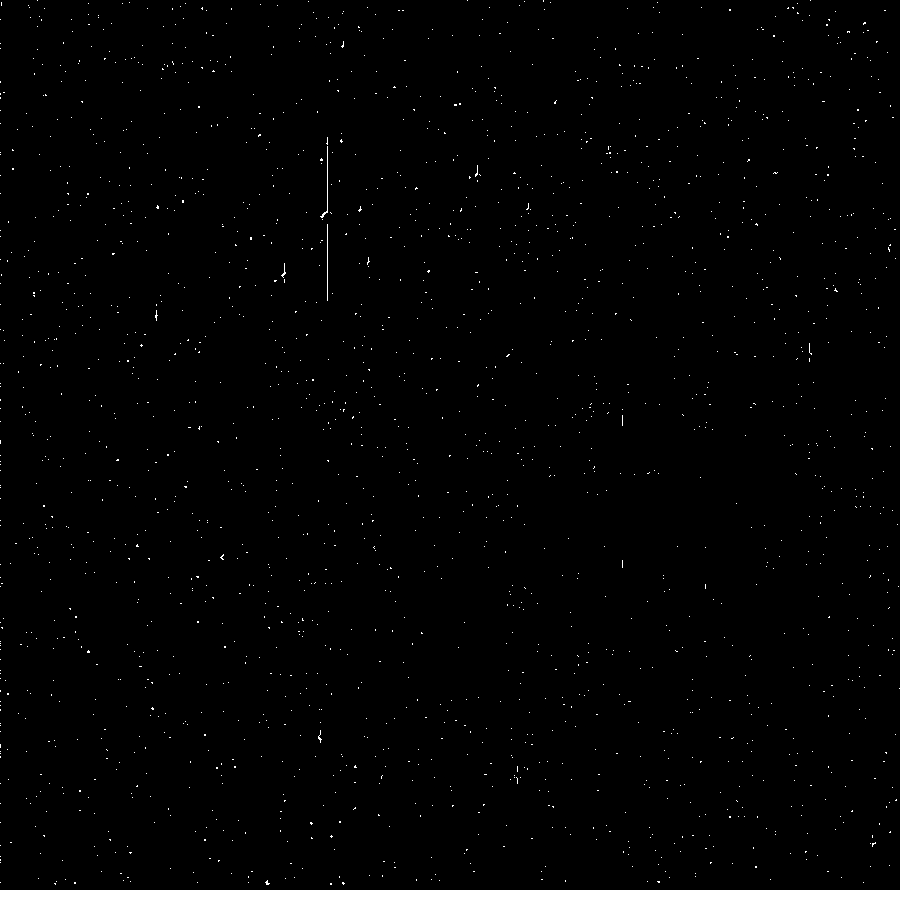
\includegraphics[width=\imgWidth]{Figures/ImageDiff_CSS3.pdf} 
%\end{array}$
%\end{center}
%\vspace{-0.7cm}
%\caption[caption]{Image Processing Pipeline results shown on Catalina Sky Survey data. 
%(row 1):  input image triplet taken approx. 10 minutes apart. 
%(row 2): Image Registration. Left: Image-1 registered to Image-2. Right: Image-3 registered to Image-2. 
%%\\\hspace{\textwidth} 
%(row 3): Image Differencing results }
%%\\\hspace{\textwidth} 
%\label{IPP_Catalina_Layout1}
%\end{figure}



%\begin{figure}[h]
%%\minipage{0.40\textwidth}
%%  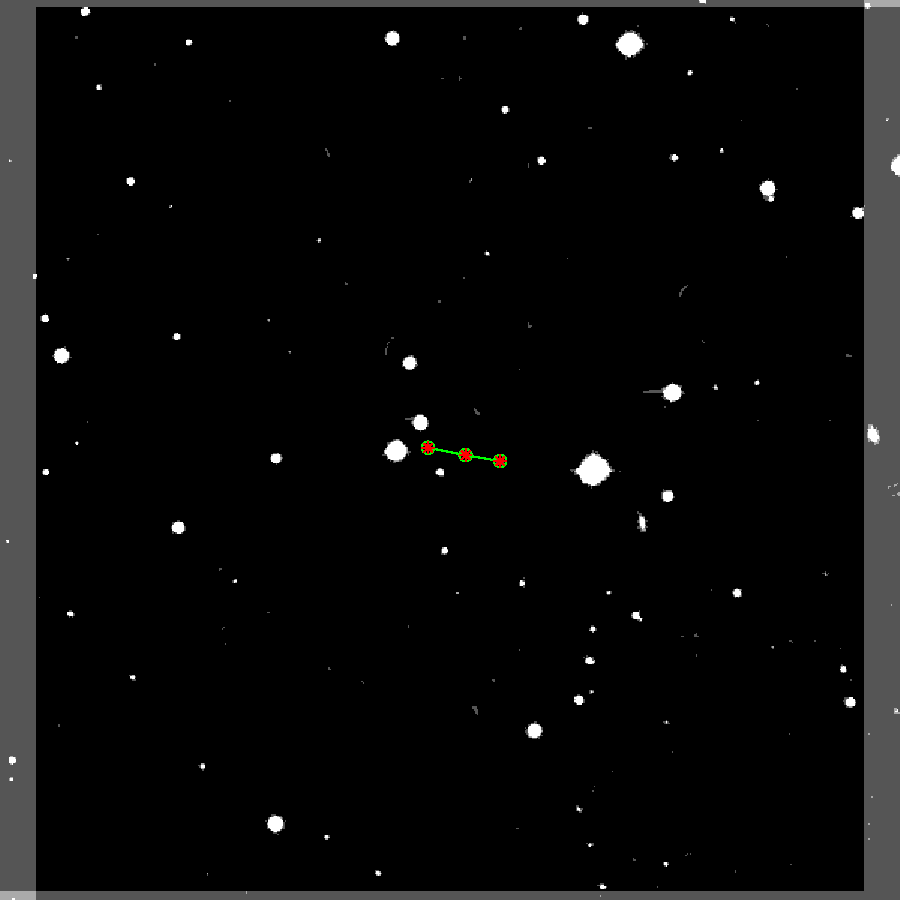
\includegraphics[width=\linewidth]{Figures/NEATLines_LogicalImg.pdf}
%%\endminipage\hfill
%\vspace{-0.7cm}
%\begin{center}
%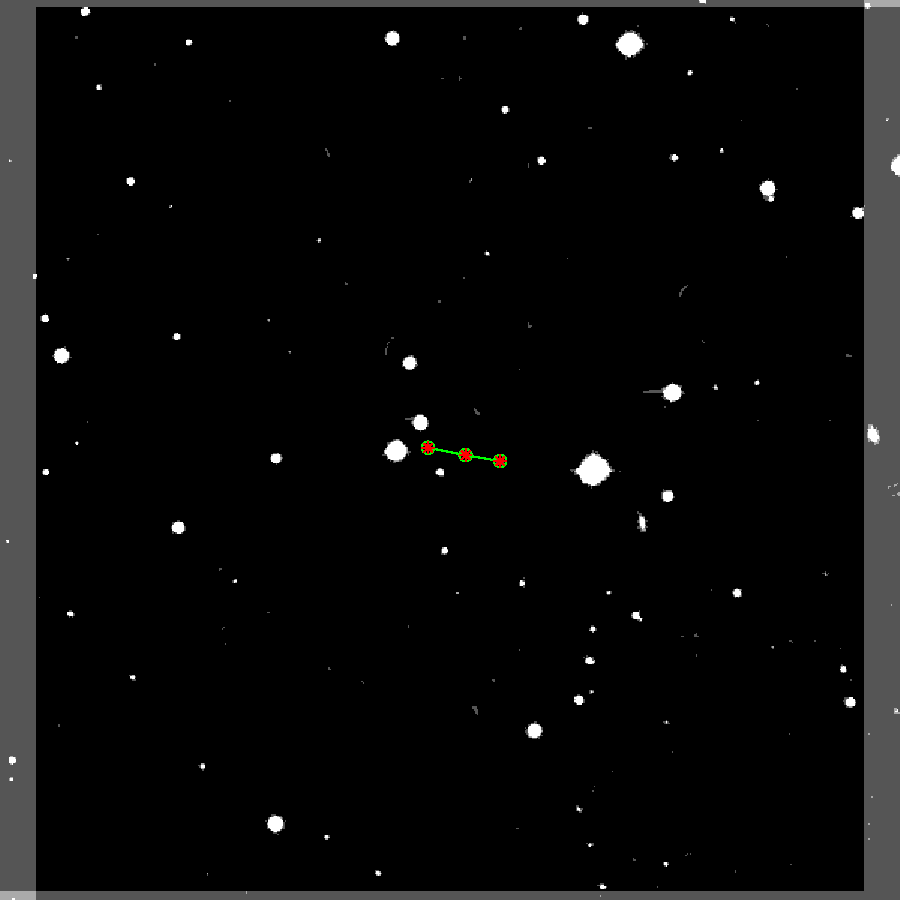
\includegraphics[width=0.4\textwidth]{Figures/NEATLines_LogicalImg.pdf}
%\end{center}
%\vspace{-0.7cm}
%\caption{Trajectory Detection for the CSS Triplet. Asteroid trajectory detected is shown in green. True location is in red. 3 Images of the triplet are super-imposed here after registration and thresholding for ease of visualization.}
%\label{fig:IPP_CSS_Trajectory}
%\vspace{-0.3cm}
%\end{figure}

\newcommand{\imgWidthMedium}{0.23\textwidth}
\begin{figure*}[h]
\begin{center}$
\begin{array}{c@{\hspace{.5em}}c@{\hspace{0.5em}}c@{\hspace{0.5em}}c}
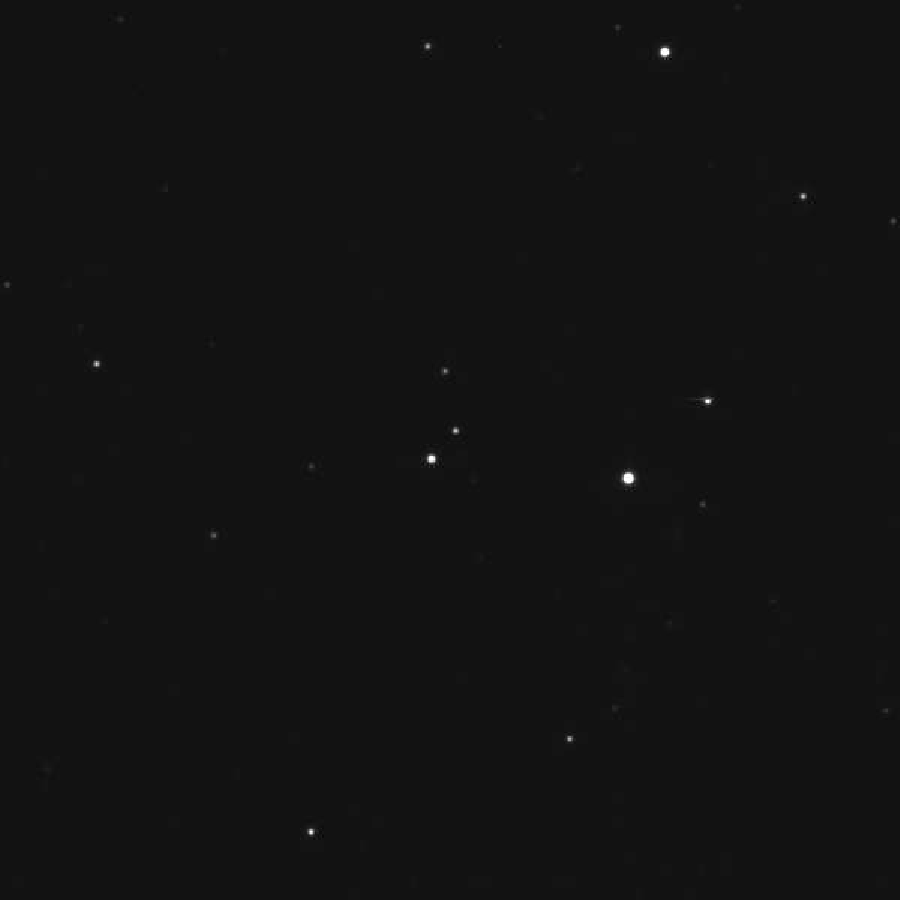
\includegraphics[width=\imgWidthMedium]{Figures/NEAT1.pdf} &
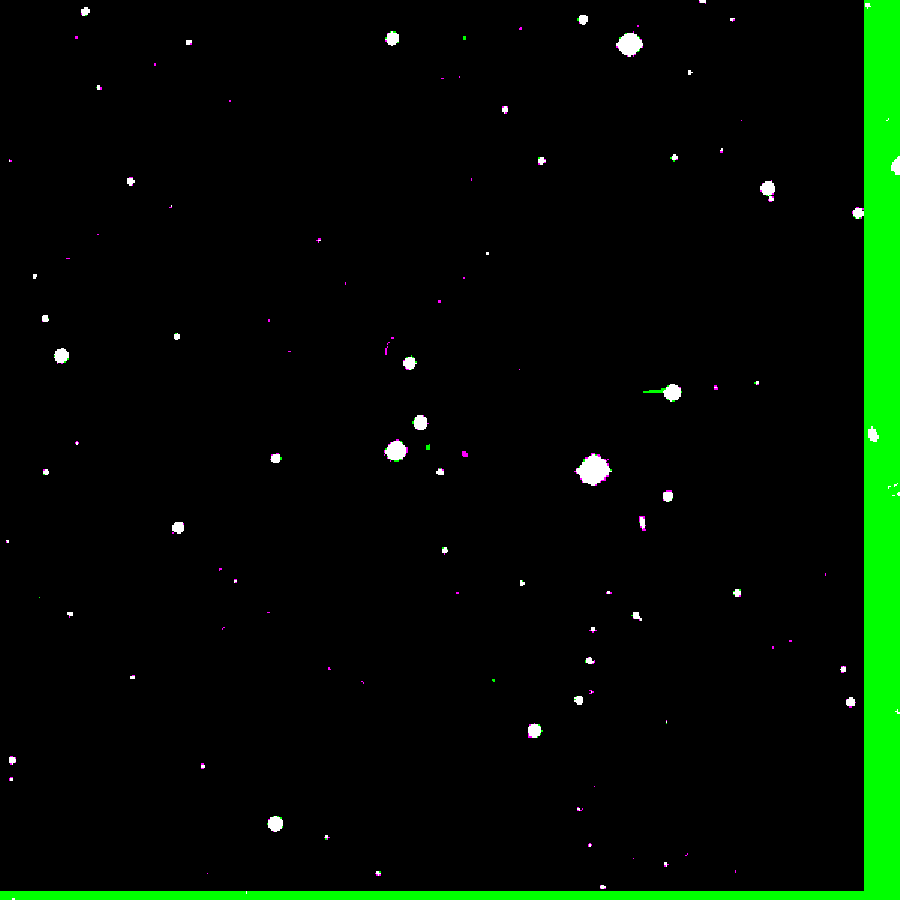
\includegraphics[width=\imgWidthMedium]{Figures/NEATImageReg12.pdf} &
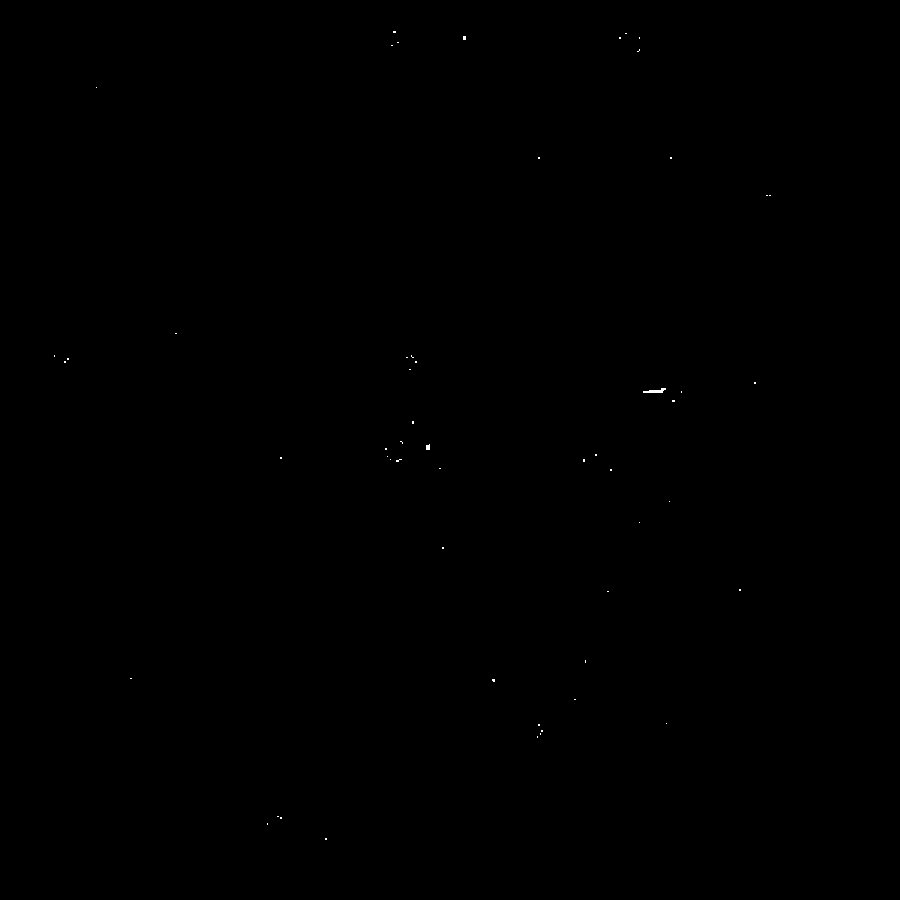
\includegraphics[width=\imgWidthMedium]{Figures/NEATImageDiff1.pdf} &
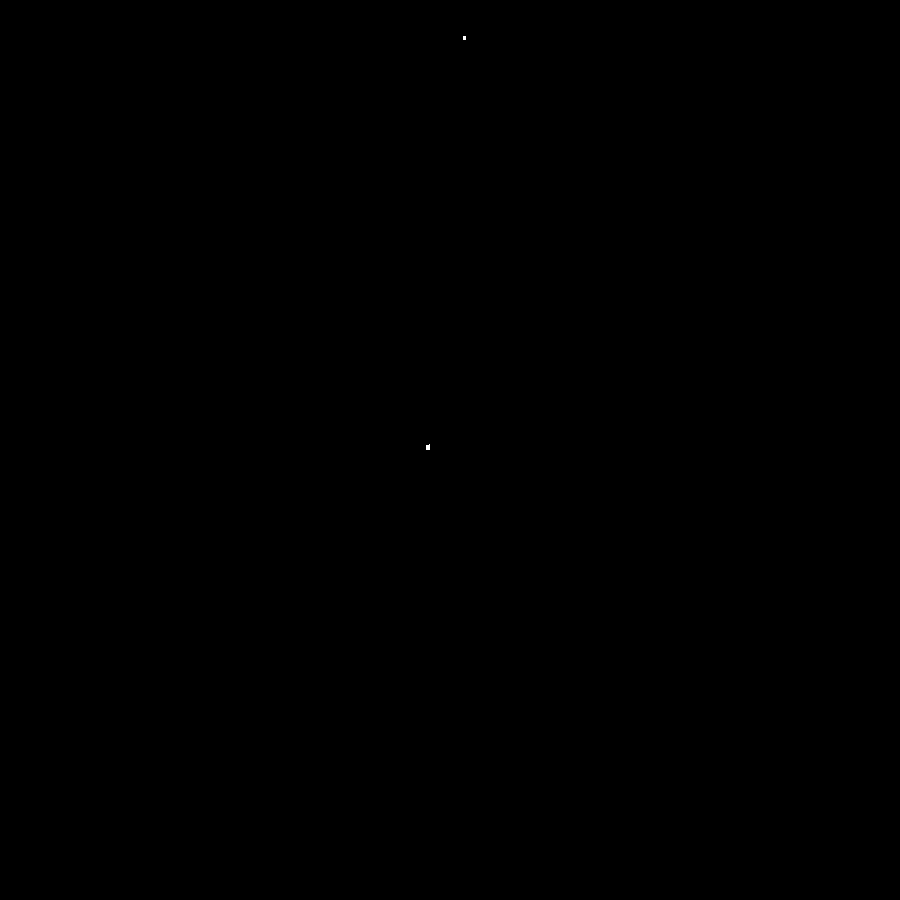
\includegraphics[width=\imgWidthMedium]{Figures/NEATFilteredCentroids1.pdf} \\
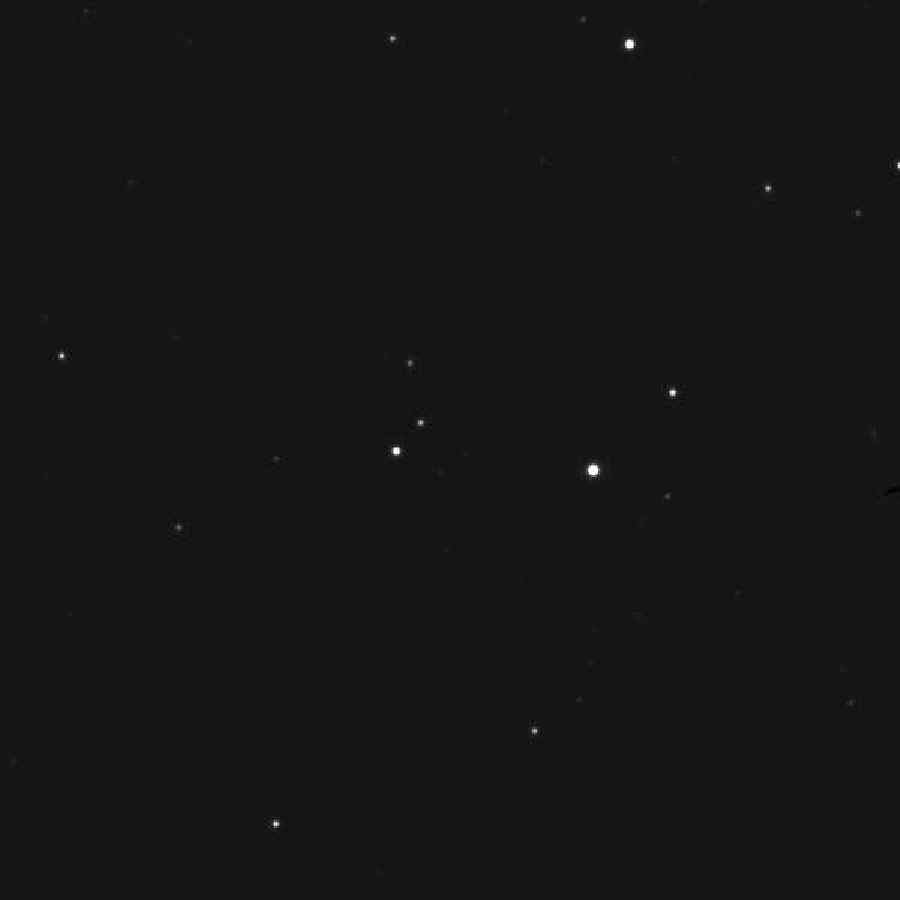
\includegraphics[width=\imgWidthMedium]{Figures/NEAT2.pdf} &
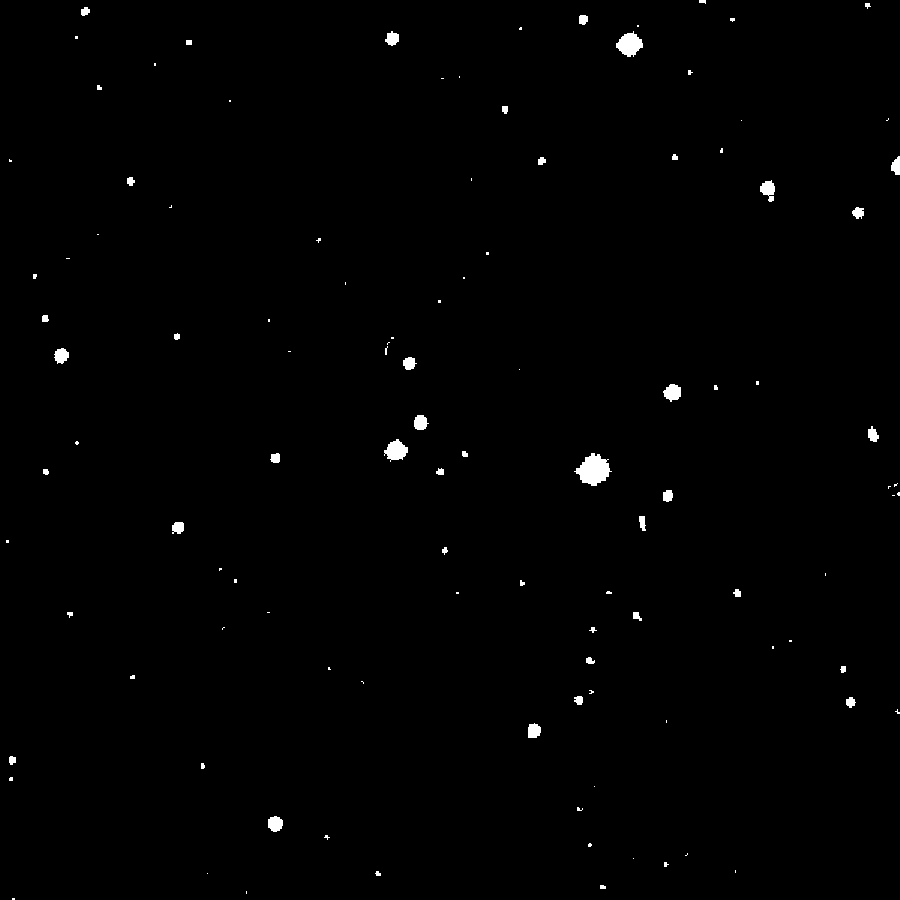
\includegraphics[width=\imgWidthMedium]{Figures/NEATImageReg22.pdf} &
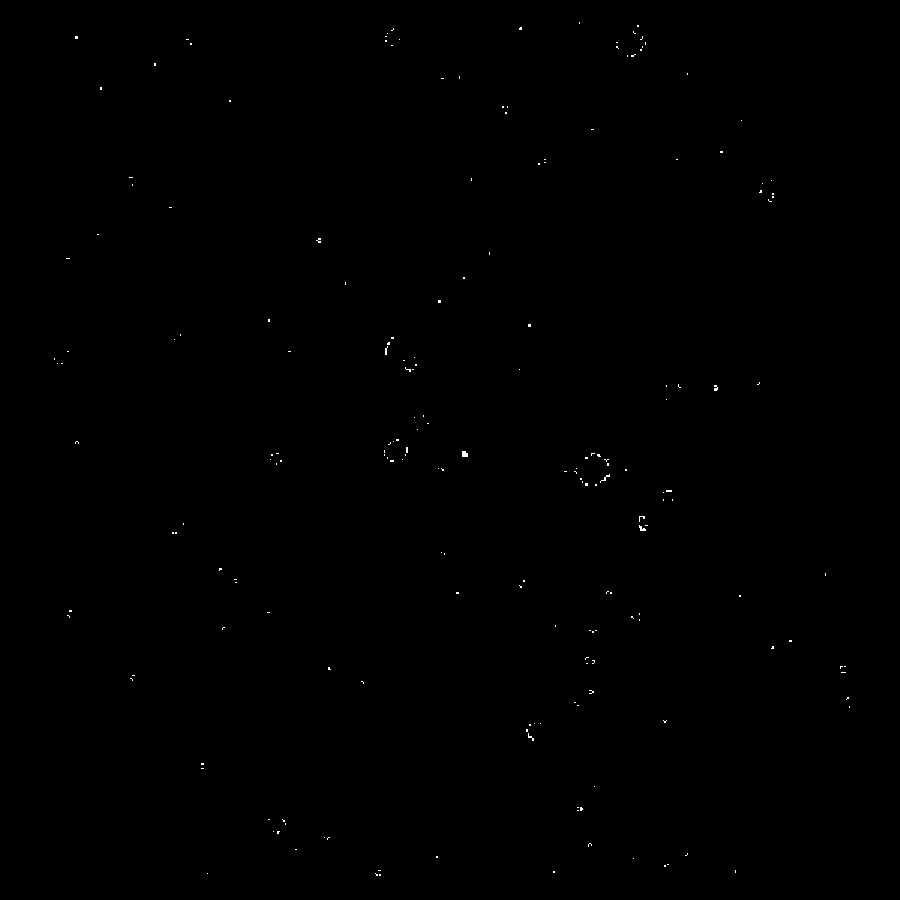
\includegraphics[width=\imgWidthMedium]{Figures/NEATImageDiff2.pdf} &
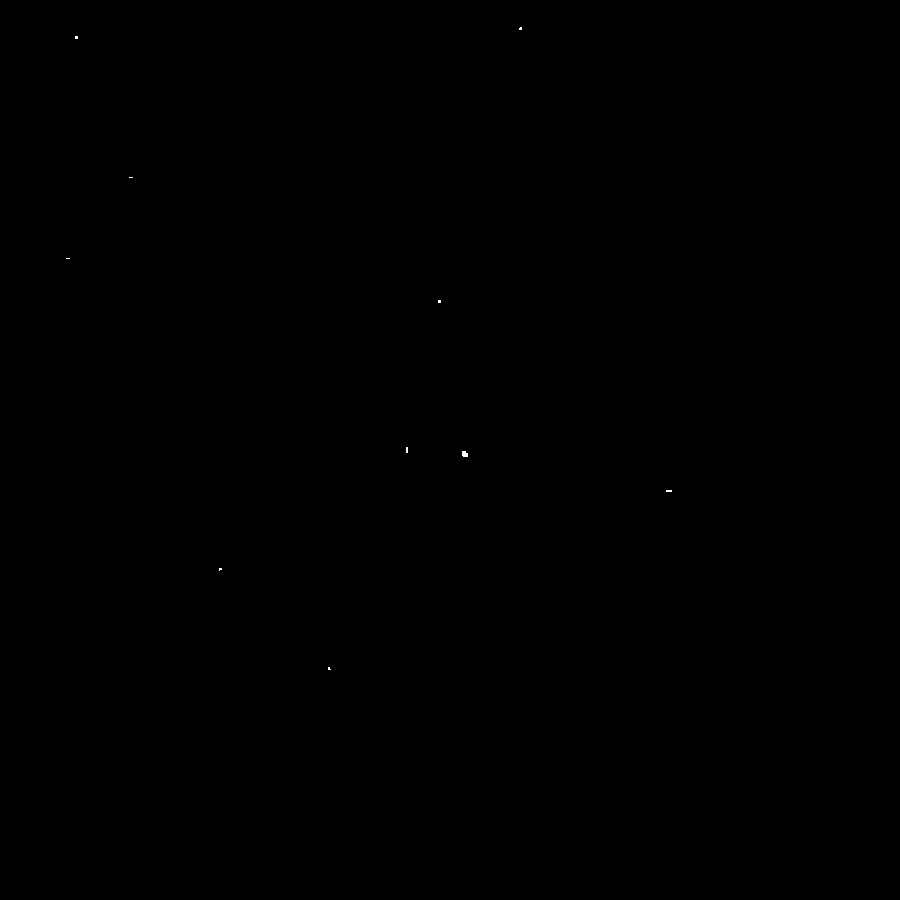
\includegraphics[width=\imgWidthMedium]{Figures/NEATFilteredCentroids2.pdf} \\
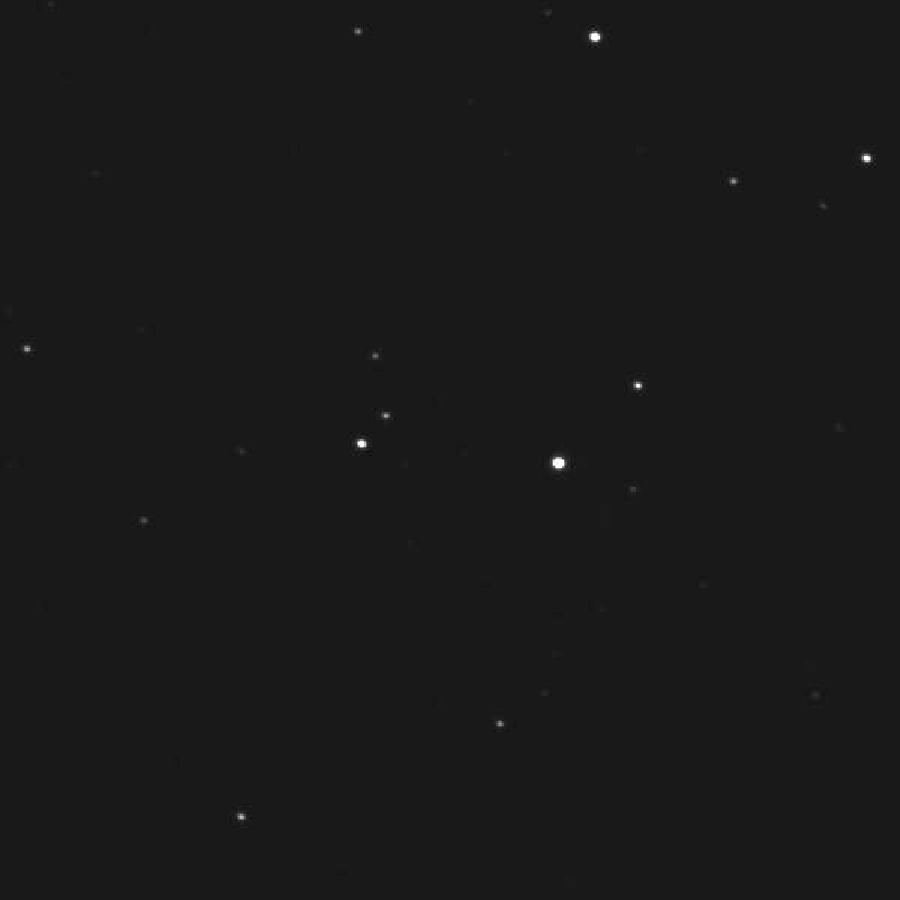
\includegraphics[width=\imgWidthMedium]{Figures/NEAT3.pdf} &
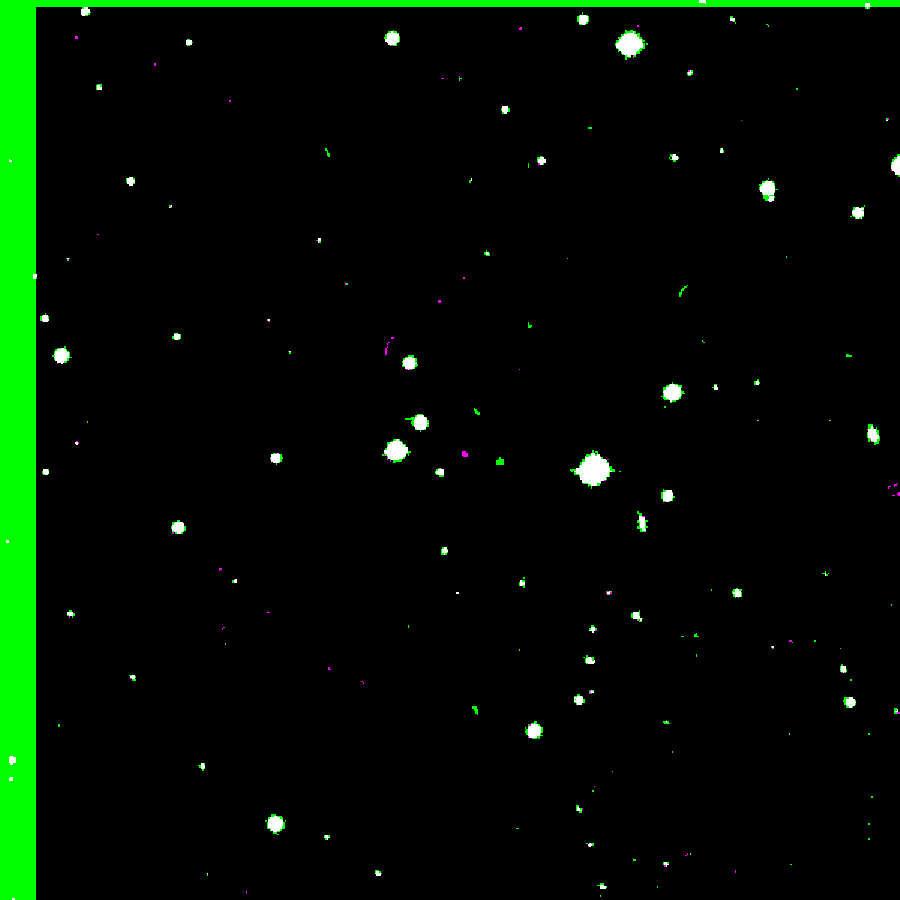
\includegraphics[width=\imgWidthMedium]{Figures/NEATImageReg32.pdf} &
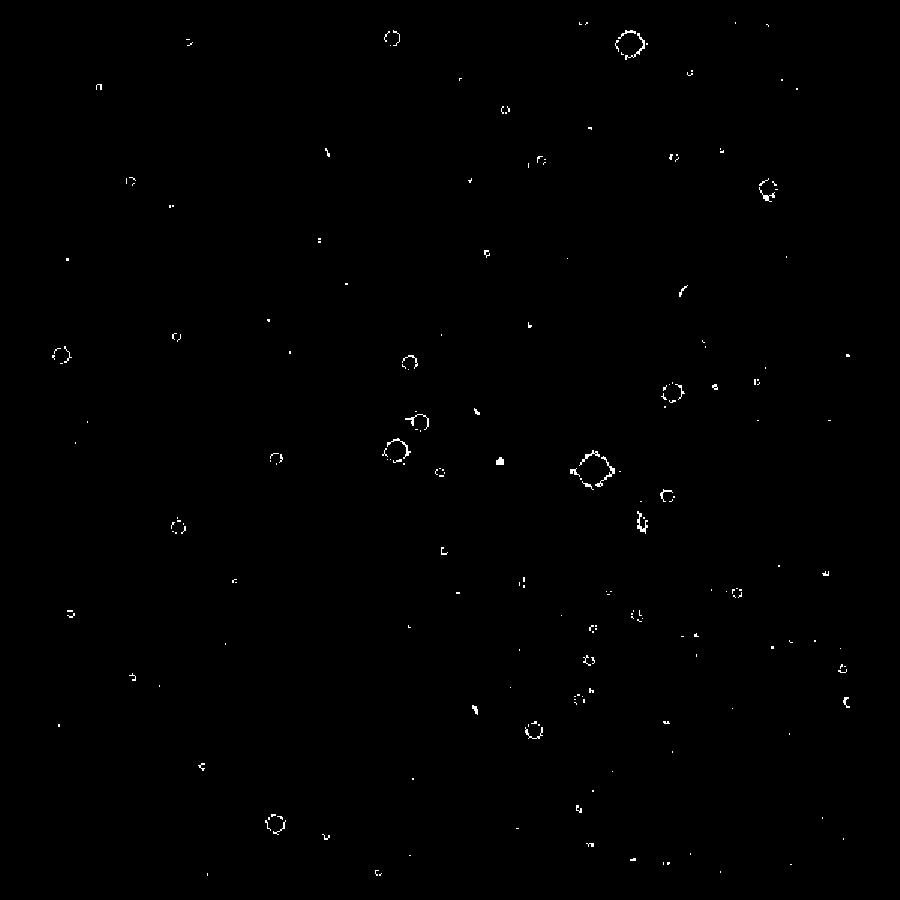
\includegraphics[width=\imgWidthMedium]{Figures/NEATImageDiff3.pdf} &
\includegraphics[width=\imgWidthMedium]{Figures/NEATFilteredCentroids3.pdf} 
\end{array}$
\end{center}
\vspace{-0.7cm}
\caption[caption]{Image Processing Pipeline results for the CY46 Triplet. (column 1): 2002 CY46 Triplet images taken approximately 10 minutes apart. Near Earth Asteroid Tracking (NEAT) system archive. 
%\\\hspace{\textwidth} 
(column 2): Image Registration results for the CY46 Triplet.  Top: Image-1 registered to Image-2. Middle: Image-2 Bottom: Image-3 registered to Image-2. 
(column 3): Image Differencing results for the CY46 Triplet. (Artifacts such as crater-like formations are seen in the difference images above. This is the result of some celestial bodies being over-exposed.) 
(column 4): Image Differencing results for the CY46 Triplet. Filtered centroids in each image of the sequence.)}
\label{IPP_NEAT_Layout2}
\end{figure*}

%\begin{figure*}[h]
%\begin{center}$
%\begin{array}{ccc}
%\includegraphics[width=0.33\textwidth]{Figures/NEAT1.pdf} &
%\includegraphics[width=0.33\textwidth]{Figures/NEAT2.pdf} &
%\includegraphics[width=0.33\textwidth]{Figures/NEAT3.pdf} \\
%\includegraphics[width=0.33\textwidth]{Figures/NEATImageReg12.pdf} &
%\includegraphics[width=0.33\textwidth]{Figures/NEATImageReg22.pdf} &
%\includegraphics[width=0.33\textwidth]{Figures/NEATImageReg32.pdf} \\
%\includegraphics[width=0.33\textwidth]{Figures/NEATImageDiff1.pdf} &
%\includegraphics[width=0.33\textwidth]{Figures/NEATImageDiff2.pdf} &
%\includegraphics[width=0.33\textwidth]{Figures/NEATImageDiff3.pdf} \\
%\includegraphics[width=0.33\textwidth]{Figures/NEATFilteredCentroids1.pdf} &
%\includegraphics[width=0.33\textwidth]{Figures/NEATFilteredCentroids2.pdf} &
%\includegraphics[width=0.33\textwidth]{Figures/NEATFilteredCentroids3.pdf}
%\end{array}$
%\end{center}
%\caption[caption]{Image Processing Pipeline results for the CY46 Triplet. 
%First row: 2002 CY46 Triplet images taken approximately 10 minutes apart. Near Earth Asteroid Tracking (NEAT) system archive. \\\hspace{\textwidth} 
%Second row: Image Registration results for the CY46 Triplet.  Top: Image-1 registered to Image-2. Middle: Image-2 Bottom: Image-3 registered to Image-2.
%\\\hspace{\textwidth}
%Third row: Image Differencing results for the CY46 Triplet. (Artifacts such as crater-like formations are seen in the difference images above. This is the result of some celestial bodies being over-exposed.) 
%\\\hspace{\textwidth}
%Fourth row: Image Differencing results for the CY46 Triplet. Filtered centroids in each image of the sequence.)}
%\label{IPP_NEAT_Layout3}
%\end{figure*}

%\begin{figure}[b]
%\minipage{0.24\textwidth}
%  \includegraphics[width=\linewidth]{Figures/NEATImageReg12.pdf}
%\endminipage\hfill
%\minipage{0.24\textwidth}
%  \includegraphics[width=\linewidth]{Figures/NEATImageReg32.pdf}
%\endminipage\hfill
%\caption{Image Registration results for the CY46 Triplet.  Left: Image-1 registered to Image-2. Right: Image-3 registered to Image-2.}
%\label{fig:NEAT_Registration}
%\end{figure}

%\begin{figure*}
%\minipage{0.33\textwidth}
%  \includegraphics[width=\linewidth]{Figures/NEATImageDiff1.pdf}
%\endminipage\hfill
%\minipage{0.33\textwidth}
%  \includegraphics[width=\linewidth]{Figures/NEATImageDiff2.pdf}
%\endminipage\hfill
%\minipage{0.33\textwidth}
%  \includegraphics[width=\linewidth]{Figures/NEATImageDiff3.pdf}
%\endminipage
%\caption{Image Differencing results for the CY46 Triplet. (Artifacts such as crater-like formations are seen in the difference images above. This is the result of some celestial bodies being over-exposed.)}
%\label{fig:NEAT_ImgDiff1}
%\end{figure*}

%\begin{figure*}
%\minipage{0.33\textwidth}
%  \includegraphics[width=\linewidth]{Figures/NEATFilteredCentroids1.pdf}
%\endminipage\hfill
%\minipage{0.33\textwidth}
%  \includegraphics[width=\linewidth]{Figures/NEATFilteredCentroids2.pdf}
%\endminipage\hfill
%\minipage{0.33\textwidth}
%  \includegraphics[width=\linewidth]{Figures/NEATFilteredCentroids3.pdf}
%\endminipage
%\caption{Image Differencing results for the CY46 Triplet. Filtered centroids in each image of the sequence.)}
%\label{fig:NEAT_ImgDiff2}
%\end{figure*}

\vspace{-0.7cm}
\subsubsection{CATALINA}
The Catalina Sky Survey (CSS) \cite{larson1998catalina,drake2009first} is intended to discover NEOs, specifically potentially hazardous asteroids that pose risk to earth. Fig. \ref{IPP_Catalina_Layout1} 
%and Fig. \ref{fig:IPP_CSS_Trajectory} 
shows the final result for one triplet of earth-based images from CSS.
\vspace{-0.3cm}
\subsection{Implementation}
This pipeline has been developed and tested in MATLAB and has also been jointly implemented in C++ on a recent Intel processor. Preliminary benchmarking on this processor has shown that peak memory usage is of the order 92 MB. Additional preliminary studies for extrapolating CPU and memory usage on an MCP750 -- a good proxy for BAE's RAD750, an operational spacecraft processor -- have led to metrics that seem promising for a possible deployment on a spacecraft architecture. We are now conducting additional work to validate these figures including activities involving the deployment of this algorithm onto a  MCP750  in conjunction with FPGAs. 




\section{CONCLUSION}

% Below is an example of how to insert images. Delete the ``\vspace'' line,
% uncomment the preceding line ``\centerline...'' and replace ``imageX.ps''
% with a suitable PostScript file name.
% -------------------------------------------------------------------------
%\begin{figure}[t]
%
%\begin{minipage}[b]{1.0\linewidth}
%  \centering
%  \centerline{\includegraphics[width=8.5cm]{Figures/image1}}
%%  \vspace{2.0cm}
%  \centerline{(a) Result 1}\medskip
%\end{minipage}
%%
%\begin{minipage}[b]{.48\linewidth}
%  \centering
%  \centerline{\includegraphics[width=4.0cm]{Figures/image3}}
%%  \vspace{1.5cm}
%  \centerline{(b) Results 3}\medskip
%\end{minipage}
%\hfill
%\begin{minipage}[b]{0.48\linewidth}
%  \centering
%  \centerline{\includegraphics[width=4.0cm]{Figures/image4}}
%%  \vspace{1.5cm}
%  \centerline{(c) Result 4}\medskip
%\end{minipage}
%%
%\caption{some placeholder figure.}
%\label{fig:res}
%%
%\end{figure}


% To start a new column (but not a new page) and help balance the last-page
% column length use \vfill\pagebreak.
% -------------------------------------------------------------------------
%\vfill
%\pagebreak


% References should be produced using the bibtex program from suitable
% BiBTeX files (here: refs). The IEEEbib.bst bibliography
% style file from IEEE produces unsorted bibliography list.
% -------------------------------------------------------------------------
\bibliographystyle{IEEEbib}
\bibliography{asteroid}

\end{document}
